%% abtex2-modelo-trabalho-academico.tex, v-1.7.1 laurocesar
%% Copyright 2012-2013 by abnTeX2 group at http://abntex2.googlecode.com/ 
%%
%% This work may be distributed and/or modified under the
%% conditions of the LaTeX Project Public License, either version 1.3
%% of this license or (at your option) any later version.
%% The latest version of this license is in
%%   http://www.latex-project.org/lppl.txt
%% and version 1.3 or later is part of all distributions of LaTeX
%% version 2005/12/01 or later.
%%
%% This work has the LPPL maintenance status `maintained'.
%% 
%% The Current Maintainer of this work is the abnTeX2 team, led
%% by Lauro César Araujo. Further information are available on 
%% http://abntex2.googlecode.com/
%%
%% This work consists of the files abntex2-modelo-trabalho-academico.tex,
%% abntex2-modelo-include-comandos and abntex2-modelo-references.bib
%%

% ------------------------------------------------------------------------
% ------------------------------------------------------------------------
% abnTeX2: Modelo de Trabalho Academico (tese de doutorado, dissertacao de
% mestrado e trabalhos monograficos em geral) em conformidade com 
% ABNT NBR 14724:2011: Informacao e documentacao - Trabalhos academicos -
% Apresentacao
% ------------------------------------------------------------------------
% ------------------------------------------------------------------------


%%%%%%%%%%%%%%%%%%
%
% As alterações realizadas no leiaute original do abntex2 disponibilizado 
% no sharelatex adaptaram o leiaute do abntex2 aos requisitos mínimos
% para escrita de dissertações e teses customizadas para o 
% centro de informática da ufpe.
%
% Bruno Maciel <bifm@cin.ufpe.com> 20/10/2016
% Daniel Severo Estrázulas <dse@cin.ufpe.br> 19/10/2020
% Alterações realizadas para o template da biblioteca atualizado disponibilizado no site Versão 07.10.2020 (1.3) revisado pelas bibliotecárias do setor bibccen.pt@ufpe.br
%%%%%%%%%%%%%%%%%%%%%%%%%%%%%%%%%%%%%%%%%%%%%%%%%%%%%%%%%%%%%%%

\documentclass[
	% -- opções da classe memoir --
	12pt,				% tamanho da fonte
	openright,			% capítulos começam em pág ímpar (insere página vazia caso preciso)
	oneside,			% para impressão em verso e anverso. Oposto a oneside
	a4paper,			% tamanho do papel. 
	% -- opções da classe abntex2 --
	chapter=TITLE,		% títulos de capítulos convertidos em letras maiúsculas
	section=TITLE,		% títulos de seções convertidos em letras maiúsculas
	%subsection=TITLE,	% títulos de subseções convertidos em letras maiúsculas
	%subsubsection=TITLE,% títulos de subsubseções convertidos em letras maiúsculas
	% -- opções do pacote babel --
	%english,			% idioma adicional para hifenização
	french,				% idioma adicional para hifenização
	spanish,			% idioma adicional para hifenização
%	brazil,				% o último idioma é o principal do documento
	english,
	brazil,
	]{abntex2/abntex2}
	\renewcommand{\baselinestretch}{1.5} %para customizar o espaço entre as linhas do texto
% --
% SETTINGS

\usepackage{abntex2/abntex2-cin-ufpe}

% \usepackage[noframe]{showframe}
% \usepackage{showframe}

%\overfullrule=4mm %para identificar onde existem os alertas de linhas grandes mal formatada pelo LaTex, basta comentar para não aparecer a barra lateral preta na linha em questão.

\renewcommand*\arraystretch{1.2} %para customizar o espaço entre as linhas das tabelas


\usepackage{pdfpages} %para incluir pdf como páginas


% ---
% PACOTES
% ---
\usepackage{amssymb}
\usepackage{float}
\usepackage{cmap}				% Mapear caracteres especiais no PDF
\usepackage{lmodern}			% Usa a fonte Latin Modern			
\usepackage[T1]{fontenc}		% Selecao de codigos de fonte.
\usepackage[utf8]{inputenc}		% Codificacao do documento (conversão automática dos acentos)
\usepackage{lastpage}			% Usado pela Ficha catalográfica
\usepackage{indentfirst}		% Indenta o primeiro parágrafo de cada seção.
%\usepackage{color}				% Controle das cores
\usepackage{graphicx}			% Inclusão de gráficos
\usepackage{lipsum}				% para geração de dummy text
\usepackage[versalete,alf,abnt-and-type=e,abnt-etal-list=0,abnt-etal-cite=3]{abntex2/abntex2cite} 
\usepackage{multirow}
\usepackage[section]{placeins}



% -----------------------------------------------------------
% lista de abreviaturas e siglas
% início
% -----------------------------------------------------------
% \usepackage[noredefwarn,acronym]{glossaries} %GLOSSÁRIO
\usepackage[acronym,nonumberlist,nogroupskip,noredefwarn]{glossaries}
% \usepackage{glossary-superragged}

\newcolumntype{L}[1]{>{\raggedright\let\newline\\\arraybackslash\hspace{0pt}}m{#1}}
\newcolumntype{C}[1]{>{\centering\let\newline\\\arraybackslash\hspace{0pt}}m{#1}}
\newcolumntype{R}[1]{>{\raggedleft\let\newline\\\arraybackslash\hspace{0pt}}m{#1}}

\newglossarystyle{modsuper}{%
  \glossarystyle{super}%
  \renewcommand{\glsgroupskip}{}
  
  % put the glossary in a longtable environment:
 \renewenvironment{theglossary}%
  {
    \begin{longtable}
        {L{0.2\textwidth}L{0.8\textwidth}}}%
    {\end{longtable}
  }%
}

% -----------------------------------------------------------
% lista de abreviaturas e siglas
% fim
% -----------------------------------------------------------


\usepackage{lscape} 
\usepackage{rotating} %rotates the figures, page
\usepackage{tikz}
\usepackage[section]{placeins}
\usepackage{setspace} 



% ----------------------------------------------------------
% PERSONALIZAÇÃO DE CORES
% ----------------------------------------------------------
\definecolor{blue}{RGB}{41,5,195}
\definecolor{gray}{rgb}{.4,.4,.4}
\definecolor{gray}{rgb}{.4,.4,.4}
\definecolor{pblue}{rgb}{0.13,0.13,1}
\definecolor{pgreen}{rgb}{0,0.5,0}
\definecolor{pred}{rgb}{0.9,0,0}
\definecolor{pgrey}{rgb}{0.46,0.45,0.48}
\definecolor{lightgray}{rgb}{0.95, 0.95, 0.96}
\definecolor{whitesmoke}{rgb}{0.96, 0.96, 0.96}
\definecolor{javared}{rgb}{0.6,0,0} % for strings
\definecolor{javagreen}{rgb}{0.25,0.5,0.35} % comments
\definecolor{javapurple}{rgb}{0.5,0,0.35} % keywords
\definecolor{javadocblue}{rgb}{0.25,0.35,0.75} % javadoc
\definecolor{meucinza}{rgb}{0.5, 0.5, 0.5}
%\definecolor{lightgray}{gray}{0.9}


% ----------------------------------------------------------
% PERSONALIZAÇÃO DO USUÁRIO
% ----------------------------------------------------------

% ----------------------------------------------------------
% DADOS DO TRABALHO - CAPA e FOLHA DE ROSTO
% Configure os dados do trabalho aqui
% ----------------------------------------------------------
\titulo{Extensão espaço-tempo-simétrica da mecânica quântica: Intepretação e previsões do tempo de chegada.}
\autor{RUBEN ESTECHE ARAÚJO}
\local{Recife}
\data{\Year}
\areaconcentracao{\textbf{Área de Concentração}: Fundamentos da Mecânica Quântica}
\orientador{\textbf{Orientador}: Prof. Dr. Eduardo Olímpio
Ribeiro Dias
}

\instituicao{UNIVERSIDADE FEDERAL DE PERNAMBUCO \\ DEPARTAMENTO DE FÍSICA - CCEN \\PROGRAMA DE PÓS-GRADUAÇÃO EM FÍSICA}
\departamento{Centro de Texto}
\programa{Pós-graduação em Física}
\emailprograma{posgrad.df@ufpe.br}
\siteprograma{https://www.ufpe.br/df/\textasciitilde posgraduacao}

\tipotrabalho{Dissertação de Mestrado}
% O preambulo deve conter o tipo do trabalho, o objetivo, 
% o nome da instituição e a área de concentração 
%\preambulo{Trabalho apresentado ao Programa de Pós-graduação em Ciência da Computação do Centro de Informática da Universidade Federal de Pernambuco, como requisito parcial para obtenção do grau de Mestre Profissional em Ciência da Computação.}

%\preambuloatadefesa{Dissertação apresentada ao Programa de Pós-Graduação Profissional em Ciência da Computação da Universidade Federal de Pernambuco, como requisito parcial para a obtenção do título de Mestre Profissional em 04 de setembro de 2020.}

\preambulo{Dissertação apresentada ao Programa de Pós-Graduação em Física da Universidade Federal de Pernambuco, como requisito parcial para a obtenção do título de Mestre em Física.}

\preambuloatadefesa{Dissertação apresentada ao Programa de Pós-Graduação em Física da Universidade Federal de Pernambuco, como requisito parcial para a obtenção do título de Mestre em Física.}




\input{userlists}






% ----------------------------------------------------------
% COMPILA O ÍNDICE
% ----------------------------------------------------------
\makeindex
% ---


% ----------------------------------------------------------
% LISTA E ABREVIATURAS E SIGLAS
% ----------------------------------------------------------
%lista de siglas
\newacronym{MEC}{MEC}{Ministério da Educação}
\newacronym{UFPE}{UFPE}{Universidade Federal de Pernambuco}


\makenoidxglossaries
\renewcommand*{\glsseeformat}[3][\seename]{\textit{#1}  
\glsseelist{#2}}

\renewcommand*{\glspostdescription}{} % remove trailing dot
\renewcommand{\glsnamefont}[1]{\textbf{#1}}

\renewcommand{\familydefault}{\sfdefault}

% ----------------------------------------------------------
% GLOSSÁRIO
% ----------------------------------------------------------

\newglossaryentry{naive-bayes}
{
  name=\textit{Na{\"i}ve Bayes},
  description={},
  plural=\textit{Na{\"i}ve Bayes}
}

\newglossaryentry{hoeffding-tree}
{
  name=\textit{Hoeffding Tree},
  description={},
  plural=\textit{Hoeffding Trees}
}















\usepackage{pdfpages}
\usepackage{inconsolata}
\usepackage{listings}
\usepackage{mathrsfs}
\usepackage{amsfonts}
\usepackage{amssymb}
\usepackage{braket}
\usepackage{physics}
\usepackage{bigints}
\usepackage{bbm, dsfont}

\definecolor{cinza}{HTML}{FCF8F8}

% define formato e estilo dos elementos do tipo Codigo Fonte
\lstset{language=PHP,
basicstyle=\ttfamily\scriptsize,
%basicstyle=\ttfamily,
keywordstyle=\color{javapurple}\bfseries,
stringstyle=\color{pblue},
commentstyle=\color{javagreen},
morecomment=[s][\color{javadocblue}]{/**}{*/},
morecomment=[s][\color{gray}]{@}{\ },
numbers=left,
numberstyle=\tiny\color{black},
backgroundcolor=\color{cinza},
stepnumber=2,
numbersep=8pt,
xleftmargin=14pt,
tabsize=4,
showspaces=false,
showstringspaces=false,
breaklines=true,}

%%%%%%%%%%%%%%%%%%%%%%%%%%%%%%%%%%



\usepackage{adjustbox} % ajustar tabela ao tamanho da pagina


% ----------------------------------------------------------
% INÍCIO DO DOCUMENTO
% ----------------------------------------------------------
\begin{document}

\frenchspacing % Retira espaço extra obsoleto entre as frases.

\imprimircapa
\imprimirfolhaderosto*~
%a ficha deve ser passada pelo setor da biblioteca e sobrescrito no formato pdf

\includepdf[pages=-]{others/ficha.pdf}

%\newpage
%\input{others/ata_defesa}
%a folha de aprovação deve ser um pdf que a secretaria encaminha sem assinaturas
%basta fazer upload na basta others e sobrescrever

\includepdf[pages=-]{others/folha_aprovacao_original}

% ----------------------------------------------------------
% DEDICATÓRIA
% ----------------------------------------------------------
\begin{dedicatoria}
   \vspace*{\fill}
%   \centering
  % \noindent
   %\textit{\lipsum[2]} 
   Para Minha família, meu amor, meus amigos, e ao meu orientador por toda a compreensão e ensinamentos compartilhados.
   %\vspace*{\fill}
\end{dedicatoria}
% ---

% ----------------------------------------------------------
% AGRADECIMENTOS
% ----------------------------------------------------------
\begin{agradecimentos}
Primeiramente, gostaria de agradecer à minha família por todo o apoio emocional e financeiro durante essa jornada acadêmica. Agradeço ao meu pai Douglas e a minha mãe Laura, por serem meus maiores incentivadores, me ajudando assim a manter o foco. Meu irmão Gustavo, obrigado por ser tão próximo e companheiro. Eu não poderia imaginar uma família melhor do que essa nem nos meus dias mais inspirados.

Aos meus amigos de curso, Naudson, Marquinhos, Anderson, Polly e Irio, Tertius, Thiago(s), Raquel, Gustavo, João, Bruninho, Lucas, Lea, Allison, Habakuke (e muitos outros que aqui não cabem) muito obrigado por serem as melhores pessoas que eu poderia ter pedido. Não teria conseguido chegar até aqui sem a ajuda e o incentivo de vocês. Espero que possamos sempre continuar tornando leve o ambiente tão pesado em que decidimos exercer nosso ofício.

E como não poderia deixar de ser, quero agradecer à minha amada Laís. Obrigado por ser minha inspiração diária, por me motivar a buscar sempre mais conhecimento e por ser a minha fonte inesgotável de amor e carinho. Você é a minha maior inspiração para sempre buscar ser melhor, e me esforçar a ir além.

Por fim, mas não menos importante, quero agradecer à minha tia Paula e a Bruna por me receberem em sua casa durante minha graduação. Vocês foram muito especiais durante esse período da minha. Obrigado por todas as emoções, aprendizados, risadas (e muitas), por tudo. O apoio de vocês foi fundamental.


Aos meus amigos interestaduais de Fortaleza que por tanto tempo fomentaram meus sonhos Brolo, Rafa, Beto, Terso e Vitinho, agradeço do fundo do meu coração pela proximidade que independe da distância. Em especial para meu amigo mais antigo que posso recordar, que por tanto tempo me acompanha e incentiva nessa empreitada acadêmica, moldando junto comigo o cientista que me tornei, obrigado Dudu.


A toda e qualquer pessoa que pôde contribuir na minha formação como físico, em especial meu orientador de mestrado, Eduardo, e meu orientador na graduação, Wilson; e a muitos amigos queridos cujos nomes não couberam aqui, meu sincero obrigado! Não seria o profissional que sou sem a ajuda de vocês. Que essa conquista seja lembrada pertencendo a todos que me ajudaram tanto quanto ela é minha.


\end{agradecimentos}


% ----------------------------------------------------------
% EPÍGRAFE

%Epígrafe: Elemento opcional e sem título em que o (a) autor (a) apresenta uma citação relacionada ao assunto tratado no trabalho. Deve ser elaborada conforme a ABNT-NBR 10520 (Citações). As citações de até três linhas devem estar entre aspas duplas e as citações com mais de três linhas devem ser destacadas com recuo de 4 cm da margem esquerda, com letra menor que a do texto e sem as aspas. A fonte da citação deve aparecer na lista de referências.
% ---------------------------------------------------------
\vspace*{10cm}
\begin{citacao}
Time is to clock as mind is to brain. The clock or watch somehow contains the time. And yet time refuses to be bottled up like a genie stuffed in a lamp. Whether it flows as sand or turns on wheels within wheels, time escapes irretrievably, while we watch. Even when the bulbs of the hourglass shatter, when darkness withholds the shadow from the sundial, when the mainspring winds down so far that the clock hands hold still as death, time itself keeps on. The most we can hope a watch to do is mark that progress. And since time sets its own tempo, like a heartbeat or an ebb tide, timepieces don’t really keep time. They just keep up with it, if they are able. \cite{manualufpe2020}.
\end{citacao}

    \vspace*{5cm}
	
		
	
\newpage

% resumo em português
\begin{resumo}[Resumo] 
Nós interpretamos a extensão \textit{space-time-symmetrical} (STS) da mecânica quântica (MQ) proposta em \cite{Dias} e exploramos as previsões de seus estados ``espaço-condicio\\nais'' (EC) para potenciais arbitrários. Seguindo uma quantização alternativa, onde o tempo se torna um operador auto-adjunto e a posição um parâmetro, a extensão STS postula a existência de um novo estado quântico (intrínseco à partícula), $|\pmb{\phi}(x)\rangle$, definido a cada ponto no espaço. $|\pmb{\phi}(x)\rangle$ obedece à uma equação de Schrödinger EC que, na base do tempo, prevê o tempo ideal de chegada da partícula em $x$. Neste trabalho investigamos o comportamento para um potencial arbitrário da equação de autovalor do momento, que é análoga à equação de autovalor da energia na MQ usual. Verificamos que para potenciais dependentes do espaço, estados com momento bem definido dependem da posição, assim como estados com energia bem definida na MQ usual dependem do tempo para potenciais dependentes do tempo. Posteriormente, interpretamos a equação de Schrödinger EC de forma análoga à equação de Schrödinger: Dada uma função de onda EC ``inicial'', $\pmb{\phi}(t|x_0)$, a solução $\pmb{\phi}(t|x)$ é a amplitude de probabilidade da partícula chegar no instante $t$, dado que o detector é movido para uma nova posição $x$. Neste contexto, comparando $|\psi(t) \rangle$ e $|\pmb{\phi}(x)\rangle$, os quais descrevem dados estatísticos coletados em $t$ e $x$, respectivamente, concluímos que eles fornecem informações complementares. Finalmente, resolvemos a equação Schrödinger EC para um potencial arbitrário dependente do espaço e aplicamos esta solução à uma barreira de potencial. Comparando esse resultado com uma generalização da distribuição de Kijowski, concluímos que a equação de Schrödinger EC talvez deva ser reformulada para acoplar as componentes de $\pmb{\phi}(t|x)$, levando em consideração a interferência entre momentos positivos e negativos.
% \noindent %- o resumo deve ter apenas 1 parágrafo e sem recuo de texto na primeira linha, essa tag remove o recuo. Não pode haver quebra de linha.

 \vspace{\onelineskip}
    
 \noindent
 \textbf{Palavras-chaves}: Fundamentos da Mecânica quântica. Tempo de chegada quântico. Incerteza energia-tempo. Extensão espaço-tempo-simétrica da mecânica quântica.
\end{resumo}



% resumo em inglês
\begin{resumo}[Abstract]
\begin{otherlanguage*}{english}

 %\noindent
We interpret the space-time-symmetric (STS) extension of quantum mechanics (QM) proposed in \cite{Dias} and explore the predictions of its ``space-conditional'' (SC) states for arbitrary potentials. Following an alternative quantization, where time becomes a self-adjoint operator and position a parameter, the STS extension postulates the existence of a new quantum state (intrinsic to the particle), $|\pmb{\phi}(x)\rangle$, defined at each point in space. $|\pmb{\phi}(x)\rangle$ obeys a SC Schr\"odinger equation that, in the time basis, predicts the ideal arrival time of the particle at $x$. In this work, first, we investigate for an arbitrary potential the momentum eigenvalue equation, which is analogous to the energy eigenvalue equation in the usual QM. We verify that for space-dependent potentials, states with well-defined momentum depend on position, just as states with well-defined energy in the usual QM depend on time for time-dependent potentials. Next, we interpret the SC Schr\"odinger equation analogously to the Schr\"odinger equation: Given an ``initial'' SC wave function, $\pmb{\phi}(t|x_0)$, the solution $\pmb{\phi}(t|x)$ is the probability amplitude for the particle to arrive at $t$, given that one moves the detector to a new position $x$. In this context, comparing $|\psi(t)\rangle$ and $|\pmb{\phi}(x)\rangle$, which describe statistical data at $t$ and $x$, respectively, we conclude they provide complementary information. Finally, we solve the SC Schr\"odinger equation for an arbitrary space-dependent potential and apply this solution to a potential barrier. Comparing this result with a generalization of the Kijowski distribution, We conclude that the SC Schr\"odinger equation should perhaps be reformulated to couple the components of $\pmb{\phi}(t|x)$, taking into account the interference between positive and negative momenta.



   \vspace{\onelineskip} 
 
   \noindent 
   \textbf{Keywords}: Foundations of Quantum Mechanics. Quantum arrival time. Energy-time uncertainty. Space-time-symmetric extension of quantum mechanics.
 \end{otherlanguage*}
 \end{resumo}



% ----------------------------------------------------------
% LISTA DE FIGURAS
% ----------------------------------------------------------
\pdfbookmark[0]{\listfigurename}{lof}
\listoffigures*
\cleardoublepage


% ---
% LISTA DE CÓDIGOS FONTES
% ---

\pdfbookmark[0]{\lstlistingname}{lol} % caso não tenha quadros, comente esta linha 
\counterwithout{lstlisting}{chapter}



% Altera o nome padrão do rótulo usado no comando \autoref{}
\renewcommand{\lstlistingname}{Código Fonte}

% Altera o rótulo a ser usando no elemento pré-textual "Lista de código"
\renewcommand{\lstlistlistingname}{Lista de códigos}

% Configura a ``Lista de Códigos'' conforme as regras da ABNT (para abnTeX2)
\begingroup\makeatletter
\let\newcounter\@gobble\let\setcounter\@gobbletwo
  \globaldefs\@ne \let\c@loldepth\@ne
  \newlistof{listings}{lol}{\lstlistlistingname}
  \newlistentry{lstlisting}{lol}{0}
\endgroup

\renewcommand{\cftlstlistingaftersnum}{\hfill--\hfil}

\let\oldlstlistoflistings\lstlistoflistings
{
\let\oldnumberline\numberline
\newcommand{\algnumberline}[1]{Código Fonte~#1~\enspace--~\enspace}
\renewcommand{\numberline}{\algnumberline}

\begin{KeepFromToc}
%\lstlistoflistings
\end{KeepFromToc}
}
\cleardoublepage

% ---
% LISTA DE QUADROS
% ---
%\pdfbookmark[0]{\listofquadrosname}{loq} % caso não tenha quadros, comente esta linha 
%\listofquadros* % caso não tenha quadros, comente esta linha 
%\cleardoublepage



% ----------------------------------------------------------
% LISTA DE TABELAS
% ----------------------------------------------------------

%\pdfbookmark[0]{\listtablename}{lot}
%\listoftables*
%\cleardoublepage


        
  
% ----------------------------------------------------------
% LISTA E ABREVIATURAS E SIGLAS
% ----------------------------------------------------------
% \printglossary[type=\acronymtype,title={\listadesiglasname},nonumberlist]
% \printglossaries
% compile uma vez com o comando \printglossaries e depois compile novamente com o comando \printglossaries comentado para as páginas glossário e siglas serem ocultadas.

% ----------------------------------------------------------
% LISTA E ABREVIATURAS E SIGLAS
% ----------------------------------------------------------
% \setglossarystyle{modsuper}
%\printnoidxglossary[style=modsuper,type=\acronymtype,title={\listadesiglasname},nonumberlist]
% \printglossary[style=super, type=\acronymtype]
%\cleardoublepage



% ----------------------------------------------------------
% LISTA DE SIMBOLOS
% ----------------------------------------------------------
%


% ---

% ---
% inserir lista de símbolos
% ---
\begin{simbolos}
  \item[$ \gamma $] Letra grega Gama
  %\item[$ \Lambda $] Lambda
  %\item[$ \zeta $] Letra grega minúscula zeta
  \item[$ \in $] Pertence
%  \item[$ \infty$] Infinito
%  \item[$ \ge$] Maior ou Igual
  \item[$ \delta$] Delta
  \item[$ \theta$] Teta
  \item[$ \sigma$] Sigma
  \item[$ \mu$] Mi
  
\end{simbolos}
% ---




% ----------------------------------------------------------
%


% ---

% ---
% inserir lista de símbolos
% ---
\begin{simbolos}
  \item[$ \gamma $] Letra grega Gama
  %\item[$ \Lambda $] Lambda
  %\item[$ \zeta $] Letra grega minúscula zeta
  \item[$ \in $] Pertence
%  \item[$ \infty$] Infinito
%  \item[$ \ge$] Maior ou Igual
  \item[$ \delta$] Delta
  \item[$ \theta$] Teta
  \item[$ \sigma$] Sigma
  \item[$ \mu$] Mi
  
\end{simbolos}
% ---






% ----------------------------------------------------------
% SUMÁRIO
% ----------------------------------------------------------
\pdfbookmark[0]{\contentsname}{toc}
\tableofcontents*
% \begingroup\intoctrue
% \tableofcontents*
% \endgroup
\cleardoublepage

% \setcounter{page}{13}
\setcounter{tocdepth}{2}
\setcounter{table}{0}




% ----------------------------------------------------------
% ELEMENTOS TEXTUAIS
% ----------------------------------------------------------
\textual


% referencie todos os arquivos de capítulos aqui, fique a vontade para
% fazer a sua organização de diretórios

  % exemplo de organização interna de um capítulo separando por mais de um arquivo

  \chapter{Introdução}
\label{chap:intro}

 \begin{citacao}
 “Time is what we want most, but what we use worst."- Willian Penn  
 \end{citacao}

	Ainda nos dias de hoje, tempo na mecânica quântica é considerado um tema controverso, e isso se deve em parte ao fato de que existem dois tratamentos possíveis para o mesmo. Por um lado, na equação de Schrödinger, tempo não é um observável (tal qual o comportamento atribuído à posição), mas sim um parâmetro externo. O estado de um sistema quântico e a distribuição de probabilidade de uma quantidade física são condicionados em um dado instante de tempo. Por outro lado, o tempo pode ser uma quantidade mensurável na  MQ. Podemos medir o instante de tempo em que uma quantidade física assume um certo valor inicial e, enquanto o sistema evolui, medir o outro instante em que a mesma quantidade assume um dado valor final. Exemplos disso são as medições de tempo de chegada, tempo de permanência, tempo de vida, entre outros. 

	Como um instante de tempo pode ser um observável, naturalmente levanta a questão de saber se podemos incluí-lo na formulação ortodoxa da mecânica quântica. A maneira mais comum de incorporar quantidades clássicas na formulação quântica é o método de quantização canônica, que consiste em substituir os colchetes de Poisson de um par de variáveis canônicas pelos colchetes de comutação dos operadores correspondentes. Dessa forma, dado o hamiltoniano $H(q, p)$ de um sistema clássico conservativo (com nenhuma dependência temporal explícita), sempre podemos fazer uma transformação canônica de $(q, p)$ para novas variáveis canônicas $(H, T)$, onde $H$ é o hamiltoniano do sistema e $T$ sua variável conjugada, que satisfaça a equação de Hamilton

\begin{equation} \label{eq1.1}
	\frac{dT}{dt} = \{ H, T \} = \frac{\delta H}{\delta H} \frac{\delta T}{\delta T} - \frac{\delta T}{\delta H} \frac{\delta H}{\delta T} = 1.
\end{equation}

Na equação acima, perceba $T$ como um intervalo de tempo. Tomando então a quantização $ \{ H, T \} \Rightarrow 1/i \hbar [\hat{H},\hat{T}]$, onde postulamos que $\hat{H}$ e $\hat{T}$ são operadores auto-adjuntos, chegamos a um operador tempo satisfazendo a relação de comutação quântica,
\begin{equation} \label{eq1.2}
	 [\hat{H},\hat{T}] = i \hbar.
\end{equation}
Isso pode ser feito tanto na representação de Heisenberg quanto na de Schrödinger. A Eq.~(\ref{eq1.2}) nos leva à relação de incerteza,
\begin{equation} \label{eq1.3}
	 \Delta H \Delta T \ge  \frac{1}{2} \left| \left<   [\hat{H},\hat{T}]  \right> \right|. 
\end{equation}
onde $\Delta H$ e $\Delta T$ são os desvios quadráticos médios de $\hat{H}$ e $\hat{T}$ respectivamente.
    
     Contudo, já no início da construção teórica da MQ, Pauli demonstrou que a existência de um operador tempo auto-adjunto seguindo a Eq.~(\ref{eq1.2}) é incompatível com o caráter limitado ou semilimitado do espectro do hamiltoniano, como mostraremos em detalhes na seção a seguir. Em contraste à teoria quântica tradicional, que não consegue satisfazer a hermiticidade de um operador temporal e atender a relação de comutação acima apresentada, os autores na Ref. \cite{Dias} propuseram uma extensão espaço-tempo-simétrica da mecânica quântica como solução para esse problema. Nesse contexto, seguindo um processo de quantização distinto, é introduzido um operador tempo que satisfaz simultaneamente tanto a condição de hermiticidade como a de comutação canônica com um novo operador hamiltoniano.
    
    Nesta dissertação, nossa intenção será propor uma interpretação mais precisa para a extensão proposta na Ref. \cite{Dias}, comparar as suas previsões com as da MQ usual e investigar medições do tempo de travessia. Como ainda será discutido nessa introdução, o caráter condicional no tempo da mecânica quântica tradicional gera complicações nas previsões dos tempos de chegada e travessia. Na próxima seção, vamos dicutir com mais detalhes o argumento proposto por Pauli para contextualizar melhor o problema do tempo como um observável. Em seguida, vamos revisar alguns modelos existentes na literatura para tempos de chegada e de tunelamento. Esses modelos servirão para comparar com as previsões da \textit{space-time-symmetrical} (STS). 





 
 

  \section{O argumento de Pauli}
\label{motivacao}

Agora, vamos voltar nossa atenção para a abordagem matemática formal que embasa a problemática do tempo como um operador. A intenção é motivar tanto a proposta de solução da Ref. \cite{Dias} para esse problema, como também a necessidade da nossa interpretação para a extensão espaço-tempo-simétrica da Ref. \cite{Dias}. 

Vamos assumir que a construção do operador temporal na Eq.~(\ref{eq1.2}) seja válida. Nesse cenário, vamos mostrar que ao aplicarmos um operador unitário $\exp \left[i E^{\prime} \hat{T} / \hbar \right]$ com $E^{\prime} \in \mathbb{R}$, no autoestado de energia $| E \rangle$ irá produzir um novo autoestado com autovalor $E$ $-E^{\prime}$, ou seja, essa aplicação irá deslocar de $- E^{\prime}$ a energia do estado $| E \rangle$. Portanto, dado um autovalor $E \in \mathbb{R}$, podemos então escolher um $ E^{\prime} \in \mathbb{R}$ qualquer para acessar um determinado estado de energia $E$ $-E^{\prime}$ desejado.

Para começar, vamos expandir o operador exponencial acima em série de potências de forma que
\begin{equation}\label{eq1.4}
    e^{iE^\prime \hat{T}/\hbar} = \sum_{n=0}^{\infty} \frac{1}{n!} \left( \frac{iE^\prime \hat{T}}{\hbar} \right)^n .
\end{equation}
Agora aplicando o operador hamiltoniano pela esquerda, obtemos
\begin{equation}\label{eq1.5}
    \hat{H} e^{iE^\prime \hat{T}/\hbar} = \sum_{n=0}^{\infty} \frac{1}{n!} \hat{H} \left( \frac{iE^\prime \hat{T}}{\hbar} \right)^n .
\end{equation}
Para entender como o operador $\hat{H}$ atua em $\hat{T}^n$, vamos utilizar a relação de comutação (\ref{eq1.2}) para criar uma relação de recorrência envolvendo $n$ e $n-1$. Isolando então $\hat{H}\hat{T}$ na Eq.~(\ref{eq1.2}), 
\begin{equation}\label{eq1.6}
   \hat{H}\hat{T} = \hat{T}\hat{H} + [\hat{H},\hat{T}] = \hat{T}\hat{H} + i\hbar.
\end{equation}
Aplicando o operador $\hat{T}$ pela direita obtemos
\begin{equation}\label{eq1.7}
   \hat{H}\hat{T}^2 = \hat{T}\hat{H}\hat{T} + i\hbar \hat{T}
\end{equation}
e substituindo a Eq.~(\ref{eq1.6}) na Eq.~(\ref{eq1.7}) é fácil ver que 
\begin{equation}\label{eq1.8}
   \hat{H}\hat{T}^2 = \hat{T} \left( \hat{T}\hat{H} + i\hbar \right) + i \hbar \hat{T} = \hat{T}^2\hat{H} + 2i\hbar \hat{T}.
\end{equation}
Se repetirmos o mesmo procedimento de aplicar o operador temporal à direita, só que agora na Eq.~(\ref{eq1.8}), e utilizarmos Eq.~(\ref{eq1.6}), obtemos 
\begin{equation}\label{eq1.9}
     \hat{H}\hat{T}^3  = \hat{T}^2 \hat{H}\hat{T} + 2 i\hbar \hat{T}^2 = \hat{T}^2 \left( \hat{T}\hat{H} + i\hbar \right) + 2i\hbar \hat{T}^2 = \hat{T}^3\hat{H} + 3 i\hbar \hat{T}^2.
\end{equation}
À essa altura já está claro que repetindo esse procedimento $n$ vezes, obtemos
\begin{equation}\label{eq1.10}
     \hat{H}\hat{T}^n = \hat{T}^{n} \hat{H} + 2i\hbar \hat{T}^{n-1}.
\end{equation}
Portanto, podemos utilizar a relação de recorrência acima na Eq.~(\ref{eq1.5}),
\begin{equation}\label{eq1.11}
\begin{split}
    \hat{H} e^{iE^\prime \hat{T}/\hbar} & = \sum_{n=0}^{\infty} \frac{1}{n!} \left( \frac{iE^\prime}{\hbar} \right)^n \left(\hat{T}^n\hat{H} + n i\hbar \hat{T}^{n-1} \right) \\
    & = e^{iE^\prime \hat{T}/\hbar}\hat{H} - \sum_{n=1}^{\infty} \frac{E^\prime}{(n-1)!}  \left( \frac{iE^\prime \hat{T}}{\hbar} \right)^{n-1},
\end{split}
\end{equation}
ou seja, 
\begin{equation}\label{eq1.12}
     \hat{H} e^{iE^\prime \hat{T}/\hbar} = e^{iE^\prime \hat{T}/\hbar}(\hat{H} - E^\prime).
\end{equation}
Finalmente, aplicando o operador acima em $| E \rangle$, temos
\begin{equation}\label{eq1.13}
    \hat{H} e^{iE^\prime \hat{T}/\hbar}\left | E \right \rangle = e^{iE^\prime \hat{T}/\hbar} (E - E^\prime)\left | E \right \rangle = (E - E^\prime)e^{iE^\prime \hat{T}/\hbar}\left | E \right \rangle.
\end{equation}
Como queríamos provar, a aplicação do operador unitário promove um deslocamento de $-E^\prime$, que pode ser arbitrariamente grande ou também infinitesimalmente pequeno dependendo da magnitude de $-E^{\prime}$. Dessa forma, a energia pode se estender de $-\infty$ até $\infty$ continuamente, contrariando a necessidade de qualquer sistema possuir um limite inferior de energia. 

A necessidade de um limite (inferior) da energia pode ser pensada de formas diferentes, por exemplo, sabemos que os sistemas tendem para o estado de menor energia (livre). Se o hamiltoniano não é limitado por baixo, não há um mínimo global de energia e, portanto, não há estado fundamental. Dessa forma, tal sistema é capaz de cair para níveis de energia cada vez mais baixos. Em consequência, o sistema é capaz de irradiar energia infinitamente, o que é obviamente um absurdo, pois nenhum sistema físico pode conter uma quantidade infinita de energia acessível. Embora possamos descrever matematicamente tal sistema, seu comportamento não é algo que observamos no mundo real.

Dito isso, precisamos então tal qual foi dito por Pauli, abandonar fundamentalmente a ideia de um operador $\hat{T}$ que seja hermitiano e satisfaça a relação $\left[ \hat{H}, \hat{T} \right] = i \hbar$. Dessa forma, a relação de incerteza energia-tempo tem sido ressignificada, por exemplo $\Delta t$ pode ser entendido como
\begin{equation}\label{eq1.14}
    \Delta t = \frac{\sigma_{Q}}{|d \langle Q \rangle / d t|}
\end{equation}
onde $\Delta t \Delta \hat{H} \geqslant \hbar / 2$ (sendo $\Delta t$ o tempo necessário de $\langle \hat{Q} \rangle$ variar um desvio padrão), e $\hat{Q}$ e $\sigma_{Q}$ dizem respeito a um um observável quântico qualquer e seu desvio padrão, respectivamente. Esse tratamento diferenciado de $\Delta t$ implica que diferentes observáveis $\hat{Q}$ têm diferentes "incertezas" $\text{ }$temporais.

A assimetria entre tempo e os observáveis quânticos exposta através do argumento de Pauli é uma consequência do tempo não ser uma variável dinâmica, e sim um parâmetro na descrição do estado quântico. Variáveis dinâmicas, nesse sentido, se tornam operadores por serem quantidades mensuráveis de um sistema físico cujo estado é condicionado a um dado instante de tempo. Sendo assim, por décadas a ideia de que era impossível introduzir um operador temporal que fosse simultaneamente hermitiano e canonicamente conjugado ao operador de energia vingou na teoria quântica. Na última seção deste capítulo, vamos discutir brevemente a hipótese formulada na Ref. \cite{Dias}, que propõe um formalismo espaço-tempo-simétrico onde o tempo se torna um observável e posição um parâmetro. Utilizando uma quantização distinta da usual, esse operador tempo tanto comuta com $\hat{H}$ como mantém sua hermiticidade, contrariando assim o argumento de Pauli. Uma revisão detalhada desse formalismo será feita no capítulo \ref{chap:cap2}.
  
%  \input{chapters/introducao/problemahipotese.tex}
  \section{Os problemas do tempo de chegada e travessia}
\label{problems}

Muito tempo se passou após a construção do argumento de Pauli e o entendimento equivocado da comunidade científica de que a busca por operadores tempo seria fútil. Apenas na década de 1960 essa questão foi investigada novamente, e desde o inicio de 1990 esse assunto vem recebendo crescente atenção (\cite{arahabom}, \cite{allcock}, \cite{13}, \cite{MugaComplex}, \cite{halli}, \cite{livrotime1}, \cite{livrotime2}).


Atualmente, a pesquisa nessa área tem uma ênfase em resolver problemas práticos, como o aparecimento "instantâneo" $\text{ }$ de elétrons no efeito fotoelétrico (atualmente processos com duração menor que nanossegundos são considerados instantâneos  \cite{20}) e o decaimento de elementos metaestáveis. Essa área também inclui o estudo teórico do papel do tempo na mecância quântica  \cite{13}, bem como soluções gerais para o problema do tempo de chegada ou tempo de tunelamento. Almejando aprofundar um pouco mais nos problemas que serão abordados nessa dissertação, as seções seguintes serão dedicadas a realizar uma breve introdução sobre esses dois últimos problemas.


\subsection{O problema do tempo de chegada}
\label{arrival}

Considere um pacote de onda inicial $\psi (x|t_0)$ restrito à região $x < 0$. O problema do tempo de chegada consiste em prever a distribuição de probabilidade temporal para a partícula chegar à uma determinada posição $x > 0$. Em outras palavras, responder a pergunta \textit{"Qual é a probabilidade de uma partícula entrar em uma região do espaço pela primeira vez durante um determinado intervalo de tempo?”}. As abordagens existentes para este problema podem ser divididas em duas classes: (i) independente e (ii) dependente do dispositivo de medição. As distribuições da categoria (i) são intrínsecas ao estado da partícula, por isso são chamados de \textit{Ideal Time-of-Arival} (TOA ideal) (\cite{Delgado}, \cite{4}, \cite{Das2}). 

Uma abordagem comum para este problema assume que, como qualquer observável na MQ, o TOA ideal é determinado pela decomposição espectral de um operador auto-adjunto (um operador tempo), a condição inicial $\psi (x|t_0)$ e um hamiltoniano independente do aparato de medida. Por causa da objeção de Pauli, esses modelos ideais são compelidos a abdicar ou da relação de comutação canônica com o hamiltoniano ou da auto-adjunção do operador tempo \cite{livrotime1}. Dessa forma, a descrição teórica dos tempos de chegada, travessia e tunelamento permanece controversa, com inúmeras abordagens surgindo nas últimas décadas (\cite{allcock}, \cite{arahabom}, \cite{Ricardo}, \cite{when}).

Outros dois métodos tradicionais para problema do TOA ideal são a distribuição de probabilidade axiomática de Kijoswiski \cite{7} e a densidade de fluxo quântico (corrente de probabilidade) (\cite{8}, \cite{Das2}). No entanto, semelhante à abordagem que utiliza um operador tempo, essas duas formulações não são irrestritamente válidas. Por exemplo, sabe-se que o fluxo quântico pode prever probabilidades negativas, um efeito chamado refluxo quântico (\cite{Das}, \cite{9}). Falhas na distribuição de Kijowski para algumas configurações experimentais podem ser encontradas nas Refs. (\cite{when},\cite{13},\cite{14}). 

A classe (ii) de abordagens para o TOA modela o dispositivo de medição levando em consideração o fato de que, na prática, os detectores não apresentam um desempenho ideal como descrito acima. Existem inúmeras descrições teóricas do aparato de medição, por exemplo, usando potenciais complexos (\cite{MugaComplex},\cite{14},\cite{18}), o colapso da função de onda (\cite{18},\cite{20}), relógios quânticos \cite{Damborenea}, integrais de caminho (\cite{Schuss},\cite{Schuss2},\cite{Schuss3}), e o formalismo de Page e Wooters para condições de contorno absorventes \cite{pagewootters}. Vale ressaltar que esses métodos operacionais e as distribuições ideais tornam-se equivalentes em circunstâncias específicas distintas. Por exemplo, ao usar um potencial complexo que absorve idealmente a função de onda sem reflexão \cite{MugaComplex}, recupera-se a densidade de fluxo quântico.

\subsection{O problema do tempo de tunelamento}
\label{tunelamento}

 A mecânica quântica implica em uma probabilidade não nula para uma partícula transpor uma barreira de potencial maior que a energia da mesma. Prever a duração deste evento é o objetivo do estudo do tempo de tunelamento. A busca por uma definição adequada e generalizada de tempos de tunelamento para partículas massivas persiste nos dias de hoje e remonta às origens da mecânica quântica. Seu estudo começou com a descoberta do decaimento $\alpha$ no início do século 20, quando foi percebido que a partícula $\alpha$ pode escapar da barreira de potencial do núcleo, a qual seria intransponível classicamente \cite{18}.

 Atualmente, as três propostas mais tradicionais no tocante a esse problema são: o \textit{phase time} (tempo de fase) introduzido por Wigner, relacionando tempo de retardo, intervalo de interação e mudanças de fase de dispersão \cite{wigner}; o \textit{traversal time} (tempo de travessia) \cite{butlan} proposto por Buttiker e Landauer em seus estudos de tunelamento através de uma barreira modulada no tempo. Pouco tempo depois, Buttiker usou a precessão de Larmor como um relógio, identificando tempos de permanência (\textit{dwell time}), travessia e reflexão como três tempos característicos que descrevem a interação de partículas com uma barreira \cite{22}. Revisões recentes que incluem essas e outras abordagens, discutindo TOA e tempos de tunelamento de uma perspectiva moderna e unificada, podem ser encontradas em \cite{24} e \cite{25}. Outras perspectivas foram lançadas sobre essas questões através de experimentos com fótons, e revisadas em \cite{26} e \cite{21}.

  
  \section{Uma breve introdução à extensão espaço-tempo-simétrica da mecânica quântica}
\label{objetivos}

Na MQ, o tempo é um parâmetro contínuo que é usado para rotular a solução da equação de onda, já a posição de uma partícula é um operador, e portanto seu valor sob uma medição é probabilístico. Essa assimetria é às vezes atribuida ao caráter não relativístico da equação de Schrödinger. Embora parcialmente correto, este argumento é insuficiente para justificar toda a disparidade entre espaço e tempo no formalismo da MQ.

Normalmente para descrever a probabilidade de encontrar uma partícula nos referimos à região $x$ no instante $t$, porém não temos a capacidade de prever o instante exato de uma provável medição. Nesse contexto, a ideia do formalismo espaço-tempo-simétrico foi pensada inicialmente para apresentar uma forma do espaço e o tempo desempenharem papéis equivalentes, possibilitando uma descrição probabilística tanto da posição $x$ como do instante de tempo $t$ em que observamos uma partícula.

Sabemos que $\psi(x| t) = \langle x|\psi(t)\rangle$ nos dá a amplitude de probabilidade de encontrar a partícula em $x$, dado que o tempo de detecção é $t$. Providos da teoria STS que será formulada detalhadamente no Cap. 2, vamos poder nos perguntar sobre a probabilidade de encontrar a partícula entre $[x, x + dx]$ e $[t, t + dt]$. Nesse cenário, indagar sobre o estado de uma partícula em um determinado momento $t$ não faz sentido, assim como perguntar na MQ usual sobre o estado dessa partícula em uma dada posição $x$. Veremos que para manter a simetria aqui proposta, precisamos de uma função de onda do tipo $\pmb{\phi}(t| x) = \langle t|\pmb{\phi}(x)\rangle$, onde $x$ agora é um parâmetro contínuo e $t$ é o autovalor de um observável. $|\psi(t|x)|^2$ nos fornece o TOA ideal na posição $x$.

Atualmente, a extensão STS foi aplicada na Ref. \cite{Parana}, no calculo do tempo de travessia de uma barreira de potencial. Os autores resolveram analíticamente a equação "dinâmica" da extensão STS no limite de potenciais $V(x) \ll E$ e  $V(x) \gg E$, sendo $E$ a energia da partícula. Foi mostrado que o valor esperado do tempo de chegada no regime de tunelamento tem a forma de uma média de energia dos tempos clássicos adicionado de uma contribuição quântica. Em outro estudo, \cite{Ricardo}, a teoria é também utilizada para prever tempos de travessia de uma barreira de potencial, mas aqui aplicada a um experimento eletromagnético que simula o tunelamento quântico. Essa revisão demonstrou uma melhor concordância com os experimentos em comparação com os modelos de Büttiker-Landauer e o \textit{phase-time}.
    
% \input{chapters/introducao/organizacao.tex}

  \section{O que vem a seguir}
\label{proxcaps}
Agora, vejamos o que abordaremos nos próximos capítulos.


No \textbf{capítulo \ref{chap:cap2}}, apresentaremos uma revisão mais detalhada do formalismo STS e de outras distribuições temporais para o tempo de chegada: a distribuição axiomática de Kijowski e o fluxo quântico.

\begin{itemize}
  \item Seção \ref{sec:cap2intro} Revisar a distribuição de Kijowski e o fluxo quântico.  
  \item Seção \ref{sec:stsreview}: Revisar todos os aspectos matemáticos do formalismo STS.
\end{itemize}



A partir do \textbf{capítulo \ref{chap:cap3}} apresentaremos nossos resultados originais.

\begin{itemize}
  \item Seção \ref{sec:bases}: Vamos estabelecer um paralelo entre $|\psi(t) \rangle$ e $|\pmb{\phi}(x)\rangle$ nas bases de energia e momento, respectivamente.
  \item Seção \ref{sec:interpretando}: Aqui, vamos interpretar mais precisamente o formalismo STS, e discutir sua conexão com a MQ usual.

Para o \textbf{capítulo \ref{chap:cap4}}, iremos aplicar nossos resultados a problemas específicos.
 
  \item Seção \ref{sec:solVarb}: Vamos resolver a equação "dinâmica" \text{ }para o caso de um potencial $V = V(x)$  qualquer.
  \item Seção \ref{sec:comparandosol}: Por fim, vamos comparar a solução da Sec. \ref{sec:solVarb} com o modelo de Kijowski para uma partícula que atravessa uma barreira de potencial. Discutiremos a possibilidade de estender a teoria STS com o intuito de levar em consideração a interferência entre momentos positivos e negativos. 
\end{itemize}

No \textbf{capítulo \ref{chap:conclusao}}, concluímos revisando os resultados originais dessa dissertação e discutindo perspectivas de trabalhos futuros. 

  \chapter{Formalismos sobre o tempo de chegada}
\label{chap:cap2}

Neste capítulo vamos revisar os modelos de Kijowski e \textit{Quantum flux}, que são distribuições do tempo de chegada ideal, preparando assim terreno para as comparações que serão feitas no capítulo seguinte. Em seguida, vamos abordar de forma mais detalhada o formalismo matemático da teoria STS.  

%exemplo de inputs, ideal para organização e troca de posicionamento futuro é ter um elemento por arquivo
%
%usar um gerador é uma opção https://www.tablesgenerator.com/
% observação, segundo a biblioteca tableas não podem ter nenhuma linha vertical

\begin{table}[ht]
\caption{Texto Texto Texto}
\label{tbl:tabelaex}
\centering
\rowcolors{1}{}{lightgray}
\begin{tabular}{p{6cm}p{9cm}}
\hline
\multicolumn{1}{c}{\textbf{Coluna A}} & \multicolumn{1}{c}{\textbf{Coluna B}}  \\
\hline     
\textbf{coluna1} & Texto Texto Texto Texto Texto Texto Texto Texto Texto Texto Texto Texto.
\\ 

coluna2 & Texto Texto Texto Texto Texto Texto Texto Texto Texto Texto Texto Texto.              
\\ 

coluna3 & Texto \textit{Texto} Texto Texto Texto Texto Texto Texto Texto Texto Texto Texto.     
\\ \hline

\end{tabular}

  \par\medskip\ABNTEXfontereduzida\selectfont\textbf{Fonte:} Elaborada pelo autor (2020) \par\medskip
\end{table}




\section{O Fluxo Quântico e a distribuição de Kijowski}
\label{sec:cap2intro}

A definição de "chegar"\text{ }em uma região específica é complicada devido à incerteza da mecânica quântica. Conceitos bem definidos são, por exemplo, aqueles do primeiro e último cruzamento de um pacote de onda \cite{14}. Portanto, para descrever o tempo de chegada de uma partícula, é importante definir claramente o conceito de "chegar". Segundo Allcock, essa área de pesquisa é ainda mais complicada do que parece, dado que ele sugere que "é muito improvável que a mecânica quântica admita qualquer conceito de tempo de chegada ideal"\text{ }\cite{allcock}. Apesar dessas ressalvas, o tempo de chegada foi estudado em profundidade por vários autores, cada um com sua abordagem específica. Descreveremos agora, em um pouco mais de detalhes, duas abordagens consideradas tradicionais sobre o tempo de chegada.




\subsection{O Fluxo Quântico}
\label{sub:fluxoquantico}


O fluxo quântico de probabilidade (também conhecido como corrente de probabilidade para o caso unidimensional) é um conceito que remonta aos primórdios da MQ, e essa grandeza advém do comportamento probabilístico da mesma. A conexão do fluxo quântico com o tempo de chegada na MQ pode ser explicada mais simplesmente  para o caso onde a probabilidade da partícula ser encontrada dentro de uma região $G$ diminui monotonicamente com o tempo. Para satisfazer esse requisito é suficiente que a função de onda $\psi(x|t)$ da partícula pertença ao conjunto
\begin{equation}\label{eqJ1}
	C^+ := \{ \psi | \textbf{j}_{\psi} (\mathbf{x}, t) \cdot d \textbf{S} \geqslant 0, \forall \text{ } \mathbf{x} \in \partial G, \forall t \geqslant 0\},
\end{equation}
onde 
\begin{equation}\label{eqJ2}
  \mathbf{j}_{\psi} (\mathbf{x}, t) = \frac{\hbar}{2m} \mathrm{Im}\left( \psi^*(\mathbf{x}| t) \nabla \psi(\mathbf{x}| t) \right)
\end{equation}
é a corrente de probabilidade, $\partial G$ é a região de contorno de $G$, e $d \textbf{S}$ é um elemento de superfície apontando para fora. 


Nessas condições específicas, define-se a probabilidade de que a partícula atravesse (chegue em) $\partial G$ depois do tempo $t$, $\mathcal{P}$(depois de $t$), como a probabilidade da partícula estar dentro de $G$ no instante $t$, $\int_G |\psi (\mathbf{x}|t)|^2 d^3 \mathbf{x}$. Portanto, a probabilidade da partícula chegar em $\partial G$ durante o intervalo de tempo $dt$ é calculada seguindo
\begin{eqnarray}\label{eqJ3}
    \Pi_j (\mathbf{x},t) dt &=& \mathcal{P}(\text{depois de } t + dt) - \mathcal{P}(\text{depois de } t) \nonumber\\ &=& \int_G |\psi(\mathbf{x}|t + dt)|^2 d^3 \mathbf{x} - \int_G |\psi(\mathbf{x}|t)|^2  d^3 \mathbf{x}\nonumber\\
        &=& \frac{d}{dt} \left( \int_G |\psi (\mathbf{x}| t)|^2 d \mathbf{x} \right)dt = \left( \int_{\partial G} \textbf{j}_{\psi} (\mathbf{x}, t) \cdot d\textbf{S} \right)dt.
\end{eqnarray}
 Note que na ultima igualdade utilizamos a equação de continuidade da probabilidade, e vemos que a densidade de probabilidade temporal da partícula chegar na area $\partial G$ é igual a $\int_{\partial G} \textbf{j}_{\psi} (\mathbf{x}, t) \cdot d\textbf{S}$, o fluxo quântico. Apesar de ser um dos modelos mais tradicionais do tempo de chegada ideal, a expressão acima tem um problema com sua interpretação probabilística, visto que $\Pi_{j} (\mathbf{x},t)$ pode admitir valores negativos em um longo, mas ainda finito, intervalo de tempo \cite{Das2}, efeito este denominado \textit{backflow effect}. Existem algumas alternativas conhecidas para contornar esse problema, as duas principais são: (i) a adoção de operadores semidefinidos positivos no espaço de Hilbert usual (o que constitui um \textit{positive operator-valued measure} --- POVM). Dado que qualquer medição quântica pode ser descrita por um POVM, a intenção dessa solução é buscar um POVM que concorde com a expressão da Eq.~(\ref{eqJ3}) para o conjunto de funções de onda da Eq.~(\ref{eqJ1}) \cite{4}. Contudo, existem classes de funções de onda que não permitem essa descrição para sua corrente de probabilidade. (ii) A segunda alternativa é a utilização de trajetórias bohmianas visto que nessa formulação as partículas possuem trajetórias bem definidas, contornando assim o problema de \textit{backflow} \cite{Das}. 
 
 Note que para o caso unidimensional $\Pi_j (x,t) = j_{\psi} (x,t)$. Considerando que a partícula é detectada em um tempo finito, a expressão deve ser normalizada. Para evitar probabilidades negativas, define-se a distribuição temporal de chegada em $x_A$ como
\begin{equation}\label{eqJ4}
\Pi (x_A,t) = \frac{|\Pi_{j} (x_A,t)|}{\int^{\infty}_{-\infty} dt |\Pi_{j} (x_A,t)|}.
\end{equation}
 Embora a validade dessa expressão ainda seja objeto de debate, ela representa um dos modelos mais tradicionais na descrição de uma medida ideal de tempo de chegada. 

% \subsection{Potencial Complexo}
% \label{sub:outrasubsection1b}




% O potencial complexo é uma ferramenta matemática usada na mecânica quântica visto sua capacidade de interagir com um sistema que tenha seu comportamento determinado por parte real e uma parte imaginária. A parte imaginária do potencial complexo pode estar relacionada à absorção ou emissão de partículas, enquanto a parte real descreve o movimento das partículas nesse sistema. A relação entre o potencial complexo e a distribuição dos tempos de chegada pode ser entendida considerando a equação de Schrödinger dependente do tempo, que descreve a evolução de um sistema quântico ao longo do tempo. Quando uma partícula está sujeita a um potencial complexo, a função de onda da partícula geralmente será modificada tanto em amplitude quanto em fase à medida que ela se move através desse tipo de potencial.


% Como argumentamos anteriormente, a fase da função de onda pode ser usada para determinar o tempo de chegada da partícula em um ponto específico do espaço. Especificamente, a fase da função de onda pode ser usada como um relógio para medir o tempo que a partícula leva para chegar a um ponto específico no espaço. Ao introduzir um potencial complexo na equação de Schrödinger, podemos determinar o efeito do potencial na função de onda e, portanto, a distribuição dos tempos de chegada. Especificamente, a parte imaginária do potencial complexo modificará a fase da função de onda, enquanto a parte real modificará a amplitude da função de onda. Essa modificação da função de onda pode ser usada para determinar a distribuição dos tempos de chegada em uma determinada posição.


% A introdução dessa ferramenta no tratamento temporal da mecânica quântica se deu através dos trabalhos de Allcock [1] usando uma função degrau puramente imaginária na sua forma mais simples como $V(x) = -i V_0 \Theta(x).$ Atualmente, é bem estabelecido que nessa abordagem, grandes valores de $V_0$ apresentarão altas taxas de reflexão (consequência do efeito Zeno) enquanto para pequenos valores onde $V_0$ tende a 0, a partícula será completamente absorvida, mas em um intervalo de espaço tão grande que resultará em uma deformação na forma de um atraso no tempo de chegada da densidade de probabilidade.


% A construção desse formalismo se baseia na definição de uma probabilidade de não detecção/absorção de uma partícula cruzando o ponto x = 0 durante um intervalo de tempo $\left[ 0, \tau \right]$ como sendo $N (\tau) = \langle \psi(\tau)|\psi(\tau)\rangle$. Portanto, definimos a probabilidade de detecção de forma que
% \begin{equation}\label{eq1}
%    N (\tau = \infty) = 1 - \int_{0}^\tau dt \Pi(t)
% \end{equation}

% Ou seja, o fluxo de probabilidade da partícula cruzar $x=0$ em um intervalo de tempo arbitrário $\left[ \tau, \tau + d\tau \right]$ é definido pela derivada $\Pi(\tau) = - d N/d\tau$ , então a partir da equação de continuidade que definimos anteriormente da equação de Schrödinger, perceba que
% \begin{equation}\label{eqcomp1}
%      \frac{\partial \rho(x,t)}{\partial t} = - \frac{\partial J}{\partial x} + \frac{1}{\hbar} V_c (x) \rho (x,t)
% \end{equation}
% onde mais uma vez $\rho(x,t) = |\psi (x,t)|^2$ e $V_c$ equivale a parte complexa do nosso potencial. Perceba que se $V_c(x) = 0$ para $x<0$ e $x<L$, podemos definir a expressão anterior entre 0 e $L$ no caso de termos um potencial complexo absorvedor ideal como sendo
% \begin{equation}\label{eq2}
%     \frac{d N^+}{d t} =  J(0,t) + \frac{1}{\hbar} <V_c>
% \end{equation}
% onde $N^+$ é a norma para $x>0$, $N^+ \equiv \int_0^L \rho (x) dx$, isto é, $N^- \equiv \int_{-\infty}^0 \rho (x) dx = - J (0,t)$. Como é fácil ver, se definirmos $N = N^+ + N^-$, 
% \begin{equation}\label{eq2}
%     \Pi(\tau) = - \frac{d N}{d\tau} = \frac{1}{\hbar} <V_c (x)> =\frac{1}{\hbar} \int \rho(x,t) V_c(x) dx.
% \end{equation}

% Para a comparação que queremos realizar aqui, iremos utilizar o modelo proposto em [3] para potenciais complexos considerando dois dos potenciais propostos naquele artigo; primeiro, usaremos o modelo proposto por Muga et al de um potencial de absorção ideal que garante mais de $99,9\%$ de absorção dentro de um intervalo arbitrário, correspondendo a um potencial não constante em $x$ que pode ser escrito como
% \begin{equation}\label{eq3}
%   V(x) = \begin{cases}
%        0, & \text{for } x < 0\\
%        p_{0}^{2} + 2(x-1)^{-1} \left( x + \frac{1}{1 + i p_{0}} \right)^{-1}, & \text{for } 0< x<1\\
%        \infty, & \text{for } x > 1
%         \end{cases}
% \end{equation}
% e também vamos considerar um potencial constante que, dados os parâmetros do nosso problema, garante uma absorção de $87,9\%$ da nossa onda na forma de $V(x) = -i V_0, \text{onde } V_0=2 .$ No contexto dessa comparação, o segundo potencial (constante) representa uma versão mais física de um experimento, dado a impossibilidade de construção de um potencial que atue como absorvedor ideal. As distribuições que calculamos para os potenciais complexos são normalizadas tomando 
% \begin{equation}\label{eq4}
%     \Pi(\tau)_{\text{norm}} = \left. \int - \frac{d N}{d\tau}  \tau d\tau \right/ \int - \frac{d N}{d\tau} d\tau. 
% \end{equation}


% Visto que assim como o modelo do Fluxo de probabilidade, $\Pi(\tau)_{\text{norm}}$ fornece uma densidade de probabilidade, precisamos então utilizar o mesmo procedimento para obter uma função de onda com o formato $ \phi (t|0)$ (tirando a raiz quadrada da sua condição inicial e multiplicando-a por uma fase complexa) para compará-lo com o STS espaço condicionado.


\subsection{O Modelo Axiomatico de Kijowski}
\label{sub:kijows}

Em uma tentativa de compreender melhor a relação entre tempo e energia na MQ, Kijowski \cite{Kijo} desenvolveu uma distribuição de probabilidade para os tempos de chegada de partículas livres. Sua abordagem consistiu em identificar as propriedades mínimas que uma distribuição de TOA deve satisfazer no caso clássico livre e, em seguida, exigir propriedades semelhantes no regime quântico. 


Primeiramente, Kijowski provou um teorema que uma distribuição do tempo de chegada deveria obedecer: considere o conjunto de funcionais bilineares positivos contínuos $F$ de funções de onda $\psi$ restritas a momentos positivos e que são invariantes sob translações espaciais. Além disso, para qualquer $\psi$ normalizado, assuma que $\int dt F[\psi_t] = 1$, onde $\psi_t$ é o estado evoluído a partir do estado inicial $\psi_0 = \psi$. Considere também que $F[\bar{\psi}] = F[\psi]$ e que a dispersão definida como
\begin{equation}
	\int_{-\infty}^{+\infty} d t \text{ } t^2 F\left[\psi_t\right]-\left(\int_{-\infty}^{+\infty} d t \text{ } t F\left[\psi_t\right]\right)^2
\end{equation}
seja finita. Sendo assim, o teorema afirma que existe então um funcional único $F_0$ para o qual esta variância é mínima. É importante reconhecer que o valor médio $\int d t \text{ } t F[\psi_t]$ é constante sobre esta classe de funcionais. O funcional $F_0$ é representado pela expressão
\begin{equation}
	F_0[\psi] = \int \frac{d P_1 dP_2}{2\pi m} \bar{\psi}(P_1)\sqrt{P_1 P_2}\psi(P_2).
\end{equation}
 Uma vez que este funcional é definido apenas para funções com momentos positivos, as suas variáveis de integração são restritas de $0$ a infinito. 
 
 
 A densidade de probabilidade do tempo de chegada para esses estados é definida como
\begin{equation}
	\Pi_{+}^K(t) = F_0\left[\psi_t\right]=\left|\int_0^{\infty} d P \sqrt{\frac{P}{2 \pi m \hbar}} e^{-i P^2 t / 2 m \hbar} \psi(P)\right|^2 .
\end{equation}
Aqui, a média de $t$ com $\Pi_{+}^K(t)$, $\int \text{d} t \text{ } t \Pi_{+}^K(t)$, coincide com a "média" \text{ }calculada através do fluxo quântico $j_{\psi}(x,t)$. Observe também que estamos lidando com o caso livre, o que significa que a amplitude de $P$ do estado evoluído $\psi_t$ está relacionada à amplitude $P$ do estado $\psi$ no instante inicial $(t = 0)$ via
\begin{equation}
	\psi_t(P)=e^{-i P^2 t / 2 m \hbar} \psi(P).
\end{equation}


Kijowski admitiu que $\Pi_{+}^K(t)$ diz respeito apenas às partículas que incidem pela esquerda, mas que as chegadas pela direita levam, por simetria, à uma expressão análoga, $\Pi_{-}^K(t)$, definida abaixo. Dessa forma, ele concluiu que uma densidade de probabilidade total da chegada no tempo $t$ na posição $x = 0$ de uma partícula em movimento livre em uma dimensão é dada por
\begin{equation}\label{eqK1}
\Pi_\psi^K(t)=\left|\int_0^{\infty} d P \sqrt{\frac{P}{2 \pi m \hbar}} e^{-i P^2 t / 2 m \hbar} \psi(P)\right|^2+\left|\int_{-\infty}^0 d P \sqrt{\frac{-P}{2 \pi m \hbar}} e^{-i P^2 t / 2 m \hbar} \psi(P)\right|^2 .
\end{equation}
Considerando uma situação de medição confirmada, vamos impor uma normalização para essa expressão
\begin{equation}\label{eqK2}
\Pi_{K}^{N} (t) = \frac{\Pi_{+} (t) + \Pi_{-} (t)}{N_{K}},
\end{equation}
onde
\begin{equation}\label{eqK3}
N_{K} = \int_{-\infty}^{+\infty} dt \sum_{\alpha \in \{+,-\}} \Pi_{\alpha} (t).
\end{equation}





\section{A extensão STS da MQ}
\label{sec:stsreview}

Nesta seção, iremos revisar a extensão STS usando uma notação semelhante à usada em \cite{Parana}. Para facilitar a compreensão da interpretação proposta na próxima seção, vamos formular a extensão STS traçando um paralelo com conceitos básicos da MQ. Vale ressaltar que o artigo original da extensão STS \cite{Dias} é um artigo relativamente curto, portanto ainda falta uma formulação mais detalhada dessa teoria.




Como introduzimos previamente, o objetivo da extensão STS proposta na Ref.~\cite{Dias} é lidar com situações experimentais complementares àquelas envolvendo distribuições condicionadas temporalmente \textit {intrínsecas à partícula}, $|\psi(x|t)|^ 2 $. Note que podemos nos perguntar sobre a probabilidade conjunta, ${\mathcal P}(x,t)dxdt$, de encontrar a partícula em uma dada região do espaço $[x,x+dx]$ e em um certo intervalo de tempo $[t,t+dt]$. Nessas condições ${\mathcal P}(x,t)$ é igual à densidade de probabilidade de encontrar a partícula na posição $x$ dado que a observação ocorre precisamente em $t$, ${\mathcal P}(x|t )=|\psi(x|t)|^2$, vezes a densidade de probabilidade ${\mathcal P}(t)$ do sistema ser medido no instante $t$, qualquer que seja o resultado. Assim, temos
\begin{eqnarray}
\label{P1}
{\mathcal P}(x,t)dxdt={\mathcal P}(x|t){\mathcal P}(t)dxdt=|\psi(x|t)|^2{\mathcal P}(t)dxdt,
\end{eqnarray}
onde ${\mathcal P}(x,t)$ e ${\mathcal P}(t)$ não podem ser obtidos exclusivamente através de $|\psi(x|t)|^2$. Vale ressaltar que a última igualdade da Eq.~(\ref{P1}) atribui à ${\mathcal P}(x|t)$ o módulo ao quadrado de uma função complexa. Sabe-se que esta relação, juntamente com a linearidade da MQ, diferencia a teoria quântica de uma teoria clássica de probabilidade. Essas características juntas permitem a existência de probabilidades do tipo $|\psi_1(x|t)+\psi_2(x|t)|^2$, que leva ao fenômeno de interferência nas possíveis posições onde se pode encontrar uma partícula. A partir da Eq.~(\ref{P1}), Ref. \cite{Dias} define uma função de onda global $\Psi(x,t)$ cujo módulo quadrado é a distribuição de probabilidade conjunta de $x$ e $t$ , ${\mathcal P}(x,t)=|\Psi(x,t)|^2$, e é normalizável por integração no espaço e no tempo. 

Por outro lado, o teorema de Bayes permite que ${\mathcal P}(x,t)$ seja reescrito como
\begin{eqnarray}
\label{P2}
{\mathcal P}(x,t)dxdt={\mathcal P}(t|x){\mathcal P}(x)dxdt \equiv|\phi(t|x)|^2 {\mathcal P}( x)dxdt,
\end{eqnarray}
onde ${\mathcal P}(t|x)$ é a densidade de probabilidade de encontrar a partícula em $t$, dado que a medição ocorre na posição $x$. Além disso, ${\mathcal P}(x)$ é a distribuição de probabilidade das medições de posição independentemente do momento em que ocorrem. Observe que $x$ e $t$ desempenham papéis opostos na Eq.~(\ref{P2}) em comparação com a Eq.~(\ref{P1}). A última igualdade da Eq.~(\ref{P2}) é o ponto crucial da extensão STS. Essa relação conjectura que a distribuição de probabilidade temporal ${\mathcal P}(t|x)$, analogamente à distribuição espacial $P(x|t)=|\psi(x|t)|^2$, vem do módulo quadrado de uma função complexa, mas agora condicionada na posição $x$. Dessa forma, o fenômeno de interferência do instante em que uma partícula é observada surge naturalmente. A partir dessa perspectiva, a MQ ordinária não-relativística pode ser vista como uma MQ \textit{temporalmente condicionada} (TC) e a extensão STS como uma MQ \textit{espacialmente condicionada} (EC). O trabalho nessa dissertação tem como foco a função de onda EC, $\phi(t|x)$, ao invés da função de onda global $\Psi(x,t)$.





Agora, temos a intuição física para definir os elementos matemáticos da extensão STS fazendo um paralelo com a MQ usual. Na teoria quântica comum, o estado de uma partícula unidimensional sem spin é definido em um instante de tempo $t$ e pertence a um espaço de Hilbert $\mathcal{H}_{t}$. Além disso, posição é um operador atuando em ${\mathcal H}_{t}$ tal que
\begin{equation}\label{position}
{\hat {\textrm X}} |x\rangle_{t}=x|x\rangle_{t}~~{ e}~~ [{\hat {\textrm X}},{\hat {\textrm P}}]=i\hbar,
\end{equation}
onde ${_{t}\langle} x|x' \rangle_t=\delta (x-x')$ e ${\hat {\textrm P}}$ é o operador de momento. A notação $|\rangle_t$ não significa que este ket tem uma dependência temporal; em vez disso, apenas enfatiza que $|\rangle_t$ pertence a ${\mathcal H}_t$. A relação de comutação~(\ref{position}) leva ao princípio de incerteza de posição e momento, $\Delta {\hat {\textrm X}} \Delta {\hat {\textrm P}} \geq \hbar/2 $, onde $\Delta$ é a raiz quadrada do erro médio. Na representação da posição, $\hat P$ é
\begin{equation}\label{momentum}
{_t\langle } x|{\hat { P}}| x' \rangle_t=- \delta(x-x') i\hbar \frac{\partial}{\partial x^\prime} 
\end{equation}
e seu autoestado $|P\rangle_t$, com ${\hat P}|P\rangle_t= P |P\rangle_t$, é
\begin{equation}\label{autoestadoP}
|P\rangle_{t}=\frac{1}{\sqrt{2\pi \hbar}} \int_{-\infty}^{\infty} e^{iPx/\hbar} |x\rangle_{t}.
\end{equation}
Aqui, a solução da indentidade é tal que
\begin{equation}\label{identityX}
\int_{-\infty}^{\infty} dx ~|x\rangle_t \langle x|=\int_{-\infty}^{\infty} dP~ |P\rangle_t\langle P|= \mathbb{I}.
\end{equation}

A informação física sobre a posição da partícula em um instante de tempo $t$ está contida em $|\psi(t)\rangle$ via a expansão
\begin{equation}\label{expansionX}
|{\psi(t)} \rangle=\int_{-\infty}^{\infty} dx~ \psi(x|t) |x\rangle_t,
\end{equation}
que é solução da equação de Schrödinger
\begin{equation}\label{Schro}
{\hat {\textrm H}}|{\psi(t)} \rangle=i\hbar \frac{d}{dt}|{\psi(t)} \rangle,
\end{equation}
onde ${\hat {\textrm H}}$ é obtida através do Hamiltoniano clássico via a regra de quantização $(x,P) \rightarrow ({\hat {\textrm X}},{\hat {\textrm P}})$, i.e.,
\begin{equation}\label{ruleX}
H(x,P;t)=\frac{P^2}{2m}+V(x,t) ~ \rightarrow ~ {\hat {\textrm H}}({\hat {\textrm X}},{\hat {\textrm P}};t)=\frac{{\hat {\textrm P}}^2}{2m}+{\hat {\textrm V}}({\hat {\textrm X}},t).
\end{equation}


Substituindo a Eq.~(\ref{ruleX}) na representação de posição da Eq.~\eqref{Schro}, obtemos
\begin{equation}\label{Schro2}
\left[-\frac{\hbar^2}{2m}\frac{\partial^2}{\partial x^2}+V(x,t)\right] \psi(x|t)=i\hbar \frac{\partial}{\partial t}{\psi ( x|t)}.
\end{equation}
Finalmente, a probabilidade de encontrar a partícula na região $[x,x+dx]$ dado que a medição ocorre no tempo $t$ é
\begin{equation}\label{rhoX}
\rho(x|t) dx=|{_t\langle} x|\psi(t)\rangle|^2dx=\psi^{*}(x|t)\psi(x|t) dx.
\end{equation}


Agora, voltemos nossa atenção para a extensão STS proposta na Ref. \cite{Dias}. Para facilitar o entendimento, vamos formular a extensão STS seguindo os mesmos passos executados acima para a MQ tradicional. Na extensão STS, o estado de uma partícula unidimensional sem spin, $|\phi(x)\rangle$, é definido em cada posição $x$ e pertence a um espaço de Hilbert ${\mathcal H}_{x}$. O tempo é um operador ${\hat {\mathbbm T}}$ agindo sobre ${\mathcal H}_{x}$ canonicamente conjugado ao operador hamiltoniano ${\hat {\mathbbm H}}$ (que é diferente de ${\hat {\textrm H}}$ da Eq.~(\ref{ruleX})), ou seja,
\begin{equation}\label{time}
{\hat {\mathbbm T}}|t\rangle_{x} =t|t\rangle_{x}~~{ \text{e}}~~ [{\hat {\mathbbm H}}, {\hat{\mathbbm T}}]=i\hbar,
\end{equation}
onde ${_x \langle} t|t' \rangle_x=\delta (t-t')$. A relação de comutação leva à relação de incerteza energia-tempo, $\Delta {\hat {\mathbbm T}} \Delta {\hat {\mathbbm H}} \geq \hbar/2 $. Semelhante a $|\rangle_t$ na MQ, o índice $x$ não significa que $|\rangle_x$ tem uma dependência espacial, mas sim que pertence à ${\mathcal H}_x$. Essa notação não foi usada nas Refs. (\cite{Dias},\cite{Ricardo},\cite{Parana}), e foi introduzida aqui para facilitar a interpretação dos autoestados da extensão STS que discutiremos no próximo capítulo.


É importante não confundir o Hamiltoniano ${\hat {\mathbbm H}}$ atuando em ${\mathcal H}_x$ com o Hamiltoniano ${\hat {\textrm H}}$ da MQ atuando em ${\mathcal H}_t$, embora se refiram ao mesmo hamiltoniano da mecânica clássica. A diferença entre eles vem do fato de seguirem regras de quantização distintas e com isso pertencerem a diferentes espaços de Hilbert. Na representação de tempo, ${\hat {\mathbbm H}}$ é definido como
\begin{equation}\label{energy}
{_x \langle} t|{\hat {\mathbbm H}}|t\rangle_x =\delta(t-t')i\hbar \frac{\partial}{\partial t},
\end{equation}
e seu autoestado $|E\rangle_x$, ${\hat {\mathbbm H}}|E\rangle_x= E |E\rangle_x$, torna-se
\begin{equation}\label{autoestadoH}
|E\rangle_x=\frac{1}{\sqrt{2\pi \hbar}} \int_{-\infty}^{\infty}dt~ e^{-iE t/\hbar} |t\rangle_x.
\end{equation}
Neste espaço de Hilbert, a resolução da identidade é
\begin{equation}\label{identityT}
\int_{-\infty}^{\infty} dt ~|t\rangle_x\langle t|=\int_{-\infty}^{\infty} dE~ |E\rangle_x\langle E|= \mathbb{I }.
\end{equation}
Comparando as Eqs.~(\ref{position})-(\ref{identityX}) com as Eqs.~(\ref{time})-(\ref{identityT}), observamos que, assim como acontece com espaço e tempo, o momento e a energia desempenham papéis opostos em ${\mathcal H}_t$ e ${\mathcal H}_x$. Note que pela Eq.~(\ref{identityT}), $E$ pode ser a priori negativo, da mesma forma que $P$ na Eq.~(\ref{identityX}). Nesse cenário, assim como os coeficientes de $|\psi(t)\rangle$ na base $\{|P\rangle_t\}$ selecionam os possíveis momentos do sistema dependendo da situação física (definida pelo potencial e as condições iniciais e de contorno), os coeficientes de $|\phi(x)\rangle$ representados em $\{|E\rangle_x\}$ selecionam as energias do sistema. Como na própria formulação da teoria a base $\{|E\rangle_x\}$ inclui energias de menos a mais infinito, o argumento de Pauli não se aplica à extensão STS.


De forma análoga à Eq.~(\ref{expansionX}), com  $x \rightleftarrows t$, a informação física do TOA de uma partícula na posição $x$ está contida em $|\pmb{\phi}(x)\rangle$ via a expansão
\begin{equation}\label{expansionT}
|{\pmb \phi(x)} \rangle =\int_{-\infty}^{\infty} dt~ \pmb \phi(t|x) ~|t\rangle_{x},
\end{equation}
onde $\pmb{\phi}(t|x)$ é um vetor de duas componentes. Como fazemos $x \rightleftarrows t$ (e $P \rightleftarrows E$) na MQ usual para formular a extensão STS, vemos que $|\pmb \phi(x) \rangle$ deve mudar espacialmente de forma análoga a como $|\psi(t)\rangle$ evolui no tempo através da equação de Schrödinger~(\ref{Schro}). Como discutido acima, o gerador de translações temporais  ${\hat {\textrm H}}$ é obtido pela quantização do hamiltoniano clássico dada pela Eq.~(\ref{ruleX}). Portanto, para obter o gerador de translações espaciais correspondente na extensão STS, devemos aplicar as novas regras de quantização~(\ref{time}) e~(\ref{energy}) ao momento clássico, i.e.,
\begin{eqnarray}\label{ruleP}
P(t,H;x)&=&\pm \sqrt{2m\big [H-V(x,t)\big ]} \nonumber\\
\rightarrow {\hat {\mathbbm P}}({\hat {\mathbbm T}},{\hat {\mathbbm H}};x)&=&\sigma_{z} \sqrt{2m\left[{\hat {\mathbbm H}}-V(x,{\hat {\mathbbm T}})\right]}.
\end{eqnarray}
onde $\sigma_z={\textrm {diag}}(+1,-1)$. Então, para que a translação espacial de $|\pmb \phi(x)\rangle$ seja análoga à translação temporal de $|\psi(t)\rangle$, $|\pmb \phi(x)\rangle$ deve obedecer
\begin{equation}\label{SchroT}
{\hat {\mathbbm P}}|{\pmb{\phi}(x)} \rangle=-i\hbar \frac{d}{dx}|{\pmb{\phi}(x) \rangle}.
\end{equation}
A partir de agora, iremos nos referir a Eq.~(\ref{SchroT}) como a equação de Schrödinger EC. Na representação do tempo, $\{|t\rangle_x\}$ , Eq.~(\ref{SchroT}) é tal que
\begin{equation}\label{Schro2T}
\sigma_{z} \sqrt{2m\left(i\hbar\frac{\partial}{\partial t}-V(x,t)\right)}\pmb{\phi}(t|x)=-i\hbar \frac{\partial \pmb{\phi}(t,x)}{\partial x},
\end{equation}
onde 
\begin{equation}\label{solT}
 \pmb{\phi} (t|x) = 
\begin{pmatrix}
    \phi^+ (t|x) \\
    \phi^- (t|x) 
\end{pmatrix}.
\end{equation}
Análogo a $t$ na MQ usual, $x$ na extensão STS é um parâmetro contínuo que pode ser escolhido com precisão arbitrária para avaliar a amplitude de probabilidade temporal $\pmb{\phi}(t|x)$. Da mesma forma que ocorre com ${\hat {\textrm H}}$ e $t$, ${\hat {\mathbbm P}}$ e $x$ não podem satisfazer o princípio da incerteza padrão.



A partir de $\pmb{\phi}(t|x)$, obtemos a probabilidade de medir a partícula no intervalo de tempo $[t,t+dt]$, dado que a observação ocorre na posição $x$,
\begin{equation}\label{rhoT}
\rho(t|x)dt=\frac{|{_x\langle} t|\pmb{\phi}(x)\rangle|^2}{\langle \pmb{\phi}(x)|\pmb{\phi}(x) \rangle} dt=\frac{\pmb{\phi}^{\dagger}(t|x)\pmb{\phi}(t|x)}{\langle \pmb{\phi}(x)|\pmb{\phi}(x) \rangle}dt.
\end{equation}
Aqui, o símbolo $\dagger$ é o operador de transposição conjugado. Na Eq.~(\ref{rhoT}), a normalização com ${\langle \pmb{\phi}(x)|\pmb{\phi}(x) \rangle}$ é necessária já que ${\hat {\mathbbm P}}$ não é sempre hermitiano. Como resultado, a equação de Schrödinger EC~(\ref{SchroT}) não é unitária em geral. Perceba que ${\langle \pmb{\phi}(x)|\pmb{\phi}(x) \rangle}$ é a probabilidade da partícula chegar em $x$ independentemente do TOA. Embora possamos observar uma partícula em qualquer instante de tempo (admitindo que ela exista, $\langle \psi(t)|\psi(t)\rangle=1$), não podemos observá-la em qualquer posição, mesmo que esperemos por uma quantidade infinita de tempo; então $0 \leq \langle \pmb{\phi}(x)|\pmb{\phi}(x) \rangle \leq 1$ \cite{Ricardo}.



Observe que a formulação da extensão STS não envolve os estados quânticos dos detectores e/ou relógios que medem o TOA, mas apenas as propriedades da própria partícula. Dessa forma, $\pmb{\phi}(t|x)$ pode ser identificado como uma amplitude de probabilidade de um TOA ideal. Por outro lado, vale ressaltar que o formalismo de Page e Wootters considera um sistema adicional desempenhando o papel de um relógio. Além disso, a superposição temporal do formalismo de Page e Wootters refere-se à história do sistema \cite{pagewootters}. Em contraste, na extensão STS, a superposição de tempo refere-se a um único evento, o TOA da partícula.

Por fim, Ref. \cite{Dias} também resolve a Eq.~(\ref{Schro2T}) para a partícula livre, $V(x,t)=0$. Identificando $\sqrt{d/dt}$ com a derivada fracionária de Riemann-Liouville $_{-\infty}D^{1/2}_t$, que é equivalente à derivada fracionária de Caputo \cite{caputo}, temos que $_{-\infty}D^{1/2}_t \exp\\(-iwt)=\sqrt{-iw} \exp(-iwt)$. A densidade de probabilidade do tempo de chegada na posição $x$, Eq. (\ref{rhoT}), torna-se
\begin{eqnarray} \label{pd}
\rho(t|x)&=& \frac{1}{2\pi m\hbar}
\Bigg\{~{\Bigg|}\int_0^{\infty}~{\tilde \phi}^+(P)~\sqrt{P}~{
e}^{iPx/\hbar-iE_P t/\hbar}~dP{\Bigg |}^2
\nonumber\\
&+& {\Bigg |} \int_0^{\infty}~{\tilde \phi}^-(P)~\sqrt{P}~{ e}^{-iPx/\hbar -
iE_P t/\hbar}~dP{\Bigg |}^2 ~\Bigg\} \frac{1}{\langle \pmb{\phi}(x) | \pmb{\phi}(x) \rangle},
\end{eqnarray}
onde $|{\tilde \phi}^{\pm}(P)|^2$ é a densidade de probabilidade da partícula ter momento $\pm P $ (com $P>0$), dado que sua observação ocorre em uma posição $x$. A  Ref.~\cite{Dias} reconhece a Eq.~(\ref{pd}) como a distribuição normalizada de Kijowski definida na Eq.~(\ref{eqK2}) identificando ${\tilde \phi}^{\pm}(P)$ como a função de onda de momento da MQ usual, ${\tilde \psi}(\pm P)$. No entanto, como as probabilidades na extensão STS estão condicionadas à uma determinada posição, essa identificação requer uma investigação mais cuidadosa. Posteriormente, depois de comparar a MQ usual e a extensão STS nas bases de energia e momento, respectivamente, e dar uma interpretação mais precisa da extensão STS, discutiremos as consequências de assumir ${\tilde \phi}^\pm(P)= {\tilde \psi}(\pm P)$.

Finalmente, vários problemas nas propostas de um TOA ideal obtidas dentro do domínio da MQ padrão não surgem aqui na extensão STS. Por exemplo, o próprio procedimento de quantização define um operador de tempo auto-adjunto que satisfaz a relação de comutação canônica com o hamiltoniano. Além disso, diferente da densidade de corrente, a teoria STS fornece uma distribuição de probabilidade de tempo positivo definida, $\rho(t|x)$.




%Podemos descrever um estado puro de uma partícula unidimensional sem spin na mecânica quântica como $| \psi(t) \rangle$, referindo ele a um espaço de hilbert $\mathcal{H}_{x}$. Nesse contexto, o observável da posição $\hat{X}$ é tal que $\hat{X} \left | x \right \rangle = x \left | x \right \rangle$. Para obtermos a função de onda de Schrödinger, basta aplicar o estado $| \psi(t) \rangle$ na base $\left | x \right \rangle$, isto é, $\langle x | \psi(t) \rangle = \psi(x|t)$, onde utilizamos a definição de probabilidade condicional aqui devido ao caráter probabilistico da mecânica quântica, sendo assim $| \langle x | \psi(t) \rangle|^2 = |\psi (x|t)|^2$ é tal qual usualmente interpretamos: \textit{\textbf{a densidade de probabilidade de detectarmos a partícula na posição $x$ dado que a medição ocorreu no instante $t$.}}

%A definição de probabilidade condicional $P_{I}(i|j)$ utilizada consiste na probabilidade de o valor de $I$ ser $I = i$ \textbf{dado que} a variável $J$ possui valor $J = j$. Podemos então calcular a probabilidade do valor de $I$ estar dentro de um intervalo $a$ e $b$ \textit{dado que} $J = c$ como
%\begin{equation}\label{eq1.15}
%    p(a,b|c) = \int_{a}^{b} P_{I}(i|c) \text{d}i
%\end{equation}
%utilizando essa definição para estender a aplicação de probabilidades condicionais no contexto de duas variáveis aleatórias, isto é $P_{I,J} (i,j)$, devemos assumir a probabilidade das variáveis assumirem os valores $I = i \in [a,b]$ e $J = j \in [c,d]$ da seguinte maneira 
%\begin{equation}\label{eq1.16}
     %p(a,b\text{ }\& \text{ }c,d) = \int_{a}^{b} \int_{c}^{d} P_{I,J}(i,j) \text{d}i \text{d}j.
%\end{equation}

%Aproveitando estas essas definições podemos então construir uma expressão para o Teorema de Bayes. Esse teorema calcula a probabilidade de um evento acontecer com base em um conhecimento \textit{a priopri} que pode estar relacionado ao mesmo evento, de forma que
%\begin{equation}\label{eq1.17}
   %  P_{I,J}(i,j) = P_{I}(i|j) P_{J}(j), 
%\end{equation}
%isto é, a probabilidade das variáveis assumirem os valores $I = i$ \textbf{e} $J = j$ é igual à densidade de probabilidade de obtermos $I = i$ \textbf{dado que} $J = j$ multiplicada pela probabilidade da variável $J$ ser igual a $j$. O raciocínio da teoria STS consiste em perceber que a densidade de probabilidade conjunta possui simetria perante a troca de $i \text{ e } j$, ou seja, $ P_{I,J}(i,j) =  P_{J}(j|i)$. Visto que nada nos impede de trocar os papéis das variáveis $I$ e $J$ de forma que $P_{J,I}(j,i) =  P_{J}(j|i) P_{I}(i)$, constatamos que
%\begin{equation}\label{eq1.18}
 %    P_{I,J}(i,j) = P_{I}(i|j) P_{J}(j) =  P_{J}(j|i) P_{I}(i). 
%\end{equation}


%Em uma tentativa direta de espelhar simetricamente o papel do operador $\hat{X}$, precisamos agora criar um espaço de Hilbert diferente do qual utilizamos para construir o argumento de Pauli, introduzindo assim um novo estado $| \phi(x) \rangle$ em conjunto com um operador tempo $\hat{T}$, relacionando os mesmos ao que vamos chamar de espaço de Hilbert $\mathcal{H}_{T}$. Nessa nova configuração vamos considerar que os autovalores do operador $\hat{T}$ representam o tempo no qual o sistema será observado, isso nos informa que $\hat{T} \left | t \right \rangle = t \left | t \right \rangle$, ou seja: a função de onda condicional $\phi(t|x)$ agora corresponde à atuação do estado $| \phi(x) \rangle$ na base $|t \rangle$, onde mais uma vez $\langle x | \phi(x) \rangle = \phi(t|x)$. Agora, $|\phi (t|x)|^2$ será dita a \textit{\textbf{ densidade de probabilidade de detectarmos a partícula no instante $t$ dado que a medição ocorreu na posição $x$.}}

%\subsection{Equação dinâmica do STS}
%\label{sub:outrasubsection1a}

%Nós definimos até então que as quantidades que são mensuráveis para o sistema para um instante de tempo qualquer como posição, momento e energia, são conhecidas como variáveis dinâmicas. Após da construção STS o tempo é promovido para variável dinâmica e passa a ser identificado pelo operador $\hat{T}$. Para formular uma equação para a função de onda temporal nesse contexto, vamos resolver a equação análoga a equação de Schrödinger dentro do espaço de hilbert $\mathcal{H}_{T}$.

%Tradicionalmente, costumamos escrever que
%\begin{equation}\label{eq2.5}
    %H (q, p; t) = \frac{p^2}{2 m} + V (x,t) \Rightarrow H (\hat{X}, \hat{p}; t) = \frac{\hat{p}^2}{2 m} + V (\hat{X},t)
%\end{equation}
%onde podemos isolar então $\hat{p}$ na equação acima e explicitá-lo em função de $H \text{ e } V$ no intuito de substituir os operadores por suas versões "espelho" $\text{ }$que são utilizadas no formalismo STS
%\begin{equation}\label{eq2.6}
%\begin{aligned}
     %p(t, H; x) = \pm \sqrt{2m} \left( H - V(t,x) \right)^{1/2} 	\Leftrightarrow P(\hat{T}, \hat{h}; x) = \hat{\sigma}_z \sqrt{2m} \left( \hat{h} - V(\hat{T},x) \right)^{1/2}
%\end{aligned}
%\end{equation}
%aplicando então na equação de Scrödinger, obtemos nossa equação espaço-condicional
%\begin{equation}\label{eq2.7}
    %\sqrt{2m} \hat{\sigma}_z \left[ \hat{h} - V(\hat{T}, x) \right]^{1/2} | \phi(x) \rangle = - i \hbar \frac{d}{d x} | \phi (x) \rangle
%\end{equation}
%que quando aplicada em $\langle t |$, fornece
%\begin{equation}\label{eq2.8}
      %\sqrt{2m} \hat{\sigma}_z \left[ i \hbar \frac{\partial}{\partial t} - V(t, x) \right]^{1/2}  \phi(t,x)  = - i \hbar \frac{\partial}{\partial x} | \phi (t,x) \rangle.
%\end{equation}
%perceba que devido ao caráter matricial de $\hat{\sigma}_z$, nossa função de onda irá assumir o formato 
%\begin{equation}\label{eq2.9}
   % \phi (t,x) = 
%\begin{pmatrix}
   % \phi^+ (t,x) \\
   % \phi^- (t,x) 
%\end{pmatrix}
%\end{equation}
%onde $\psi^+$ representa a amplitude da partícula incidir em um sentido no aparato localizado em $x$ e $\psi^-$ no outro sentido. A densidade de probabilidade total fica então representada por 
%\begin{equation}\label{eq2.10}
   % \rho (t,x) = |\phi^+|^2 + |\phi^-|^2 = \phi^\dagger \phi.
%\end{equation}
  
    %Analogamente à forma como resolvemos a equação de movimento de partículas livres na MQ, podemos usar uma separação de variáveis na forma $\phi(t|x) = e^{-i\epsilon t/ \hbar} \phi_\epsilon (x)$, expandindo a expressão de \ref{eq2.7} em série, isto é
%\begin{equation}\label{eq2.11}
    %\hat{\sigma_z} \sqrt{2m [\epsilon - V(x)]} \phi_\epsilon (x) = -i \hbar \frac{d}{dx} \phi_\epsilon (x)
%\end{equation} 
%problema este que configura uma equação diferencial de primeira ordem com solução já conhecida por nós no formato
%\begin{equation}\label{eq2.12}
   % \phi_\epsilon (x) = \frac{1}{\sqrt{2 \pi \hbar}} e^{(i/\hbar)\hat{\sigma_z} \int_{0}^{x} \sqrt{2m [\epsilon - V(x)]} dx^{\prime}}
%\end{equation} 
%como \ref{eq2.12} ainda é uma equação linear, podemos escrever a sua solução geral, isto é, a equaçào dinâmica de movimento da teoria STs como
%\begin{equation}\label{eq2.13}
  %  \phi (t|x) = \frac{1}{\sqrt{2 \pi \hbar}} \int d\epsilon C_\epsilon  e^{(i/\hbar)\hat{\sigma}_z \int_{0}^{x} \sqrt{2m [\epsilon - V(x)]} dx^{\prime}-i\epsilon t /\hbar}.
%\end{equation}




% \section{Revisão sobre formalismos de Tempo de Tunelamento}
% \label{sec:section3}

% Não existe uma definição que seja universalmente aceita entre as conhecidas “tempo de permanência” (\textit{dwell time}), “tempo de tunelamento” (\textit{tunneling time}) ou “tempo de travessia” (\textit{transversal time}). Como Landauer coloca: “Não há direitos autorais sobre as expressões de tempo de travessia e tempo de tunelamento; cada autor pode escolher uma interpretação. Se um investigador quiser associá-lo ao tempo necessário para escrever o hamiltoniano de tunelamento de Bardeen no quadro-negro, não podemos dizer que está errado.” [13].

% No entanto, como mencionado em Damborenea et al. o “tempo de permanência” é distinto do “tempo de travessia”, “tempo de atraso” ou “tempo de reflexão” [28], e é importante entender as diferenças entre cada uma dessas abordagens e suas respectivas particularidades associadas. Vamos enfatizar então uma abordagem especifica voltada para tentar definir o “tempo de tunelamento” que julgamos melhor se encaixar no contexto de comparação com o nosso modelo. 


% \subsection{Distribuição temporal de Kijowski para Tempo de Travessia}
% \label{sub:outrasubsection1c}

% Para construir uma distribuição de probabilidade no contexto de tunelamento, isto é, quando uma barreira real é colocada antes de fazer nossa medição temporal, podemos utilizar dos mesmos axiomas propostos para formular a distribuiçào de Kijowski no caso de TOA. Definindo um funcional que atenda às condições para descrever o operador normalizado da distribuição de tempo de chegada para uma partícula tunelada, sua expressão pode ser obtida como em ref[8] ref[9],
% \begin{equation}\label{T1}
%     \Pi_{pot}^{on} (t) = \frac{1}{2 \pi m \hbar} \left| \int dk \widetilde{\psi}(k) e^{-i \hbar k^2 t / 2m + i \hbar k x} \sqrt{k} \frac{T(k)}{|T(k)|} \right|^2
% \end{equation}
% onde $T(k)$ é a amplitude do coeficiente de transmissão quântica ref[10]
% \begin{equation}\label{T2}
%     T(k) = \frac{4 k_0 k_1 e^{-i L(k_0 - k_1)}}{\left(k_0 + k_1 \right)^2 - e^{2 i L k_1} \left(k_0 - k_1 \right)^2}
% \end{equation}
% com $k_0 = \sqrt{2mE}$ e $k_1 = \sqrt{2m(E-V_0)}$. Esta expressão coincide com o proposto na ref[8] ref[9] ref[10] e também foi utilizada no contexto de comparação com o STS space na obra ref[11].

% Na configuração que vamos propor, uma partícula se aproxima de um ponto muito distante pela esquerda do potencial real, para evitar problemas envolvendo medições negativas intrinsícas a esse modelo. Como nosso objetivo é propor um regime de medição positiva no lado direito do potencial impondo a certeza de transmissão, iremos utilizar a normalização do pacote de saída usando $T(k) \widetilde{\psi}(k) / (\int dk |T(k) \widetilde{\psi}(k)|^2 )^{1/2} $ em vez de apenas usar $\widetilde{\Psi} (k)$, ou seja, iremos considerar o potencial real como
% parte do procedimento de preparação, impondo assim que a partícula irá interagir com o mesmo. A distribuição final é calculada utilizando esse fator na distribuição de Kijowski, sendo assim
% \begin{equation}\label{T3}
% \begin{split}
%     \Pi_{K}^{T} (t) & = \frac{1}{2 \pi m \hbar} \left| \int dk \widetilde{\psi}(k) e^{-i \hbar k^2 t / 2m + i \hbar k x} \sqrt{k} T(k) \right|^2\\
%     & \times \left( \int dk |T(k) \widetilde{\psi}(k)|^2 \right)^{-1}.
% \end{split}
% \end{equation}
  
  \chapter{Interpretando a extensão STS e comparando-a com a MQ}
\label{chap:cap3}

Neste capítulo, vamos explorar algumas consequências da extensão STS, fornecendo uma interpretação mais precisa das soluções de sua equação ''dinâmica'', Eq.~(\ref{SchroT}), e comparando as informações contidas em $|\psi(t)\rangle $ e $|\pmb{\phi}(x)\rangle$. Uma interpretação dos autoestados de observáveis na extensão STS também será discutida. Ressaltamos que a partir de agora os resultados apresentados são originais desta dissertação.



\section{$|\psi(t)\rangle$ na base de energia {\textit versus} $|\pmb{\phi}(x)\rangle$ na base de momento}
\label{sec:bases}

A equação de autovalor de energia na MQ usual é equivalente à equação de autovalor de momento na extensão STS. Assim, conforme investigaremos, um potencial dependente do tempo na equação de Schrödinger~(\ref{Schro}) tem um efeito análogo a um potencial dependente do espaço na equação de Schrödinger EC~(\ref{SchroT}). Dito isso, consideramos $V=V(x,t)$ para lidarmos com o caso mais geral possível. Nesta seção iremos comparar as soluções gerais $|\psi(t)\rangle$ e $|\pmb{\phi}(x)\rangle$ nas bases de energia e momento, respectivamente. Vamos começar revisando a MQ usual para um hamiltoniano dependente do tempo~\cite{sakurai}. Primeiro, os autoestados de energia intantâneos satisfazem
\begin{equation}\label{SchroE1}
{\hat {\textrm H}}(t)|E_a(t)\rangle = E_a(t)|E_a(t)\rangle,
\end{equation}
onde $a$ é uma variável contínua tal que $\langle E_{a'}(t)|E_a(t)\rangle=\delta(a'-a)$ e $\int da |E_a(t)\rangle {\langle} E_a(t)|=1$. Semelhante à $|\psi(t)\rangle$, estamos omitindo o índice $t$ em $|E_a(t)\rangle$.


Um estado arbitrário em ${\mathcal H}_t$ pode então ser expandido nesta base instantânea de energia,
\begin{equation}\label{expansion}
    \ket{\psi(t)}=\int da ~ {\bar \psi}(E_a|t) \ket{E_a(t)},
\end{equation}
onde
\begin{equation}\label{PsiE}
    {\bar \psi}(E_a|t) \equiv {\langle} E_a(t)|\psi(t)\rangle= C(a|t)e^{i \theta_a(t)},
\end{equation}
com $\theta_a(t)=-1/\hbar\int_0^t \dd{t'}E_a(t')$ sendo a fase dinâmica. Da equação de Schrödinger~(\ref{Schro}), é fácil ver que o coeficiente $C(a|t)$ satisfaz
\begin{equation}\label{Ca}
    \frac{dC(a|t)}{dt}=-\int \dd{a'} C(a'|t)e^{i\Delta \theta_{a'a}(t)}\bra{E_a(t)}\frac{d}{dt}\ket{E_{a'}(t)},
\end{equation}
onde introduzimos $\Delta \theta_{a'a}(t)=\theta_{a'}(t)- \theta_a (t)$. Observe que ${\mathcal P}(E_{a}|t)=|{\bar \psi}(E_{a}|t)|^2=|C(a|t)|^2$ ($\theta_{a}(t)$ é um número real) é a densidade de probabilidade de medir a partícula com energia $E_{a}$, dado que a medição ocorre no tempo $t$. Agora, projetando a Eq.~(\ref{expansion}) em $|x\rangle_t$ produz
\begin{equation}\label{SolX3}
\psi(x|t)={_t\langle} x|\psi(t)\rangle=\int da ~\bar{\psi} (E_a|t)  \psi_a(x|t),
\end{equation}
onde $\psi_a(x|t)={_t\langle} x|E_a(t)\rangle_t$ é a amplitude de probabilidade da partícula ser encontrada na posição $x$, dado que sua energia é $E_a$ e o observação acontece no tempo $t$. Note que o índice $a$ representa uma variável condicional de modo que $\psi(x|E_a,t)$ também seria uma notação conveniente para ${_t\langle} x|E_a(t)\rangle_t$.

Para o hamiltoniano~(\ref{ruleX}), a projeção da Eq.~(\ref{SchroE1}) em $ \ket{x}$ resulta em
\begin{equation}\label{SchroXE}
    \left[-\frac{\hbar^2}{2m}\pdv[2]{x}+V(x,t) \right]\psi_a(x|t)=E_a(t) ~\psi_a(x|t).
\end{equation}
Em particular, para a situação de partícula livre, onde $[{\hat{H}},\hat{P}]=0$, $\psi_a(x|t)={_t\langle} x|E_a(t) \rangle$ torna-se independente do tempo e é dado por
\begin{eqnarray}\label{SolXFree}
\psi_E^\pm(x)=\sqrt{\frac{m}{2\pi \hbar }}\frac{1}{(2E)^{1/2}}\exp{\pm \frac{ i\sqrt{2mE}x}{\hbar}},
\end{eqnarray}
onde $\pm$ refere-se ao sinal do momento. Além disso, ${\bar \psi}(E_a|t)$ da Eq.~(\ref{PsiE}) pode ser escrito como ${\bar \psi}^{\pm}(E|t)={\bar \psi}^{\pm}(E) e^{-iEt/\hbar}$ e a solução geral~(\ref{SolX3}) torna-se
\begin{equation}\label{SolXL}
    \psi(x|t)=\int_{0}^{\infty} dE ~ \big[{\bar \psi}^+(E) \psi_E^+(x)+{\bar \psi}^-(E)  \psi_E^-(x)\big]e^{-iEt/\hbar},
\end{equation}
com ${\mathcal P}^{\pm}(E|t)=|{\bar \psi}^{\pm}(E)|^2$ independente do tempo.








A análise equivalente na extensão STS começa com a equação de autoestado do momento,
\begin{equation}\label{SchroTP1}
\hat{\mathbb P}(x) \ket{\pmb{P}_b(x)}= P_b(x)|\pmb{P}_b(x)\rangle
\end{equation}
[analogamente à Eq.~(\ref{SchroE1})], onde
\begin{equation}\label{Pb}
\ket{\pmb{P}_b(x)}=\mqty(|P^+_b(x)\rangle   \\ |P^-_b(x)\rangle)
\end{equation}
e, novamente, $b$ é uma variável contínua onde, ${\langle} \pmb{P}_{b'}(x)|\pmb{P}_b(x)\rangle=\delta(b'-b)$ e $\int db |\pmb{P}_b(x)\rangle{\langle} \pmb{P}_b(x)|=1$. Aqui também estamos omitindo o índice $x$ nos autoestados de momento. Observe que, assim como os potenciais dependentes do tempo na MQ usual produzem auto-estados de energia dependentes do tempo, um potencial dependente do espaço na extensão STS leva a auto-estados de momento dependentes do espaço. Isso significa que os estados com momento bem definido dependem da posição em que descrevemos a partícula. Em contraste, lembre-se que as autofunções de momento (energia) na MQ usual (extensão STS) são sempre as mesmas, proporcionais a $\exp{iPx/\hbar}$ ($\exp{-iEt/\hbar}$).


Analogamente à Eq.~(\ref{expansion}), utilizando da linearidade da equação de Shrödinger EC, um estado físico arbitrário em ${\mathcal{H}}_x$ na posição $x$ pode então ser expandido na base de momento como
\begin{equation}\label{expansionT}
    \ket{{\pmb \phi}(x)}=\int db~ {\tilde \phi}(P_b|x) \ket{{\pmb P}_b(x)},
\end{equation}
onde
\begin{equation}\label{phiP}
   {\tilde \phi}(P_b|x)\equiv \langle \pmb{P}_b(x)|\pmb{\phi}(x)\rangle= C(b|x)e^{i\theta_b(x)},
\end{equation}
com $\theta_b(x)=1/\hbar\int_0^x d x^\prime P_b(x')$ sendo o equivalente à fase dinâmica $\theta_a(t)$ na MQ usual. A partir da equação de Schrödinger EC~(\ref{SchroT}), pode-se verificar facilmente que o coeficiente $C_b(x)$ satisfaz uma equação semelhante à~(\ref{Ca}),
\begin{equation}
    \frac{dC(b|x)}{dx}=-\int d{b'} C(b'|x)e^{i\Delta \theta_{b'b}(t)}\bra{\pmb{P}_b(x)}\frac{d}{dx}\ket{\pmb{P}_{b'}(x)},
\end{equation}
onde $\Delta \theta_{b'b}(x)=\theta_b'(x)-\theta_b(x)$. Agora, nós temos
\begin{equation}\label{prob}
{\mathcal P}(P_b|x)=\frac{|{\tilde \phi}(P_b|x)|^2}{{\langle \pmb{\phi}(x)|\pmb{\phi}(x) \rangle}}
\end{equation}
como a amplitude de probabilidade de medir o estado com momento $P_b$, dado que a medição ocorre na posição $x$. Observe que $e^{i \theta_b(x)}$ é relevante para a Eq.~(\ref{prob}), pois $\theta_b(t)$ pode ser um número puramente imaginário. Projetando a Eq.~(\ref{expansionT}) em $|t\rangle_x$, obtemos uma expansão análoga à Eq.~(\ref{SolX3}) para a extensão STS,
\begin{equation}\label{SolT3}
{\pmb \phi}(t|x)={_x\langle} t|\phi(t)\rangle=\int db ~{\tilde \phi}(P_b|x) {\pmb \phi}_b(t|x),
\end{equation}
onde  
\begin{equation}\label{phib}
   \pmb{\phi}_b(t|x)=\mqty({_x\langle} t|P^+_b(x)\rangle   \\ {_x\langle}t|P^-_b(x)\rangle)\equiv \mqty( \phi^+_b(t|x)   \\ \phi^-_b(t|x) )
\end{equation}
é a amplitude de probabilidade da partícula chegar no tempo $t$, dado que seu momento é $P_b(x)$ e o detector está na posição $x$. 


Agora, usando $\mathbbm P$ definido na Eq.~(\ref{ruleP}), a projeção da Eq.~(\ref{SchroTP1}) em $|t\rangle_x$ resulta em
\begin{equation}\label{SchroTP}
\sigma_z \sqrt{2m\left(i\hbar \pdv{t}-V(x,t)\right)}\pmb{\phi}_b(t|x)=P_b(x)\pmb{\phi}_b(t|x).
\end{equation}
A Ref.~\cite{Dias} analisou a equação de autovalor do momento para a situação de partícula livre, onde $[{\hat {\mathbb P}},\hat {\mathbb H}]=0$. Em nossa situação, análogo à Eq.~(\ref{SolXFree}) na MQ usual, $\pmb{\phi}_b(t|x)$ definido na Eq.~(\ref{phib}) torna-se independente do espaço, e aqui é dado por duas funções vetoriais independentes,
A Ref.~\cite{Dias} analisou a equação de autovalor do momento para a situação de partícula livre, onde $[{\hat {\mathbb P}},\hat {\mathbb H}]=0$. Nossa situação, análogo às Eqs.~(\ref{SolXFree}) na MQ usual, $\pmb{\phi}_b(t|x)$ definido na Eq.~(\ref{phib}) torna-se independente do espaço, e aqui é dado por duas funções vetoriais independentes,
\begin{equation}\label{SolTL}
    \pmb{\phi}_{P_+}(t|x)=\mqty(\phi^+_{P_+}(t|x)   \\  0)
\end{equation}
e
\begin{equation}\label{SolTL}
   \pmb{\phi}_{P_-}(t|x)=\mqty(0  \\  \phi^-_{P_-}(t|x) ),
\end{equation}
com
\begin{eqnarray}\label{SolTFree}
\phi^{\pm}_{P_{\pm}}(t|x)=\phi^{\pm}_{P_{\pm}}(t)=\sqrt{\frac{|P_\pm|}{2\pi
m\hbar}}~\exp{-\frac{i(P_\pm)^2t}{2m\hbar}}.
\end{eqnarray}
e $P_\pm=\pm \sqrt{2mE}$, onde $E$ é a energia da partícula. Além disso, ${\tilde \phi}(P_b|x)$ definido na Eq.~(\ref{phiP}) pode ser escrito como
\begin{eqnarray}\label{phiPFree}
  {\tilde \phi}(P_{\pm}|x)={\tilde \phi}(P_\pm)e^{ iP_{\pm}x/\hbar},
\end{eqnarray} 
Considerando $E>0$ e definindo $\tilde{\phi}^{\pm}(P) \equiv \tilde{\phi} (P_{\pm})$, com $P=|P_\pm|$, a solução geral~(\ref{SolT3}) torna-se
\begin{eqnarray}\label{SolTL}
    \pmb{\phi}(t|x) = \int_0^\infty dP\big[{\tilde \phi}^+(P)\pmb{\phi}_{P_+}(t) e^{iPx/\hbar} + {\tilde \phi}^-(P)  \pmb{\phi}_{P_-}(t)e^{-iPx/\hbar} \big],
\end{eqnarray}
onde seu módulo quadrado normalizado é $\rho(t|x)$ dado na Eq.~(\ref{pd}). Vale a pena notar a semelhança entre as Eqs.~(\ref{SchroXE})-(\ref{SolXL}) e as Eqs.~(\ref{SchroTP})-(\ref{SolTL}). Diferente da MQ usual, onde ${\mathcal P}(E|t)=|{\bar \psi}(E)|^2$ é independente do tempo para partículas livres, ${\mathcal P}(P_{ \pm}|x)=|{\tilde \phi}^{\pm}(P)|^2/\langle \pmb{\phi}(x)|\pmb{\phi}(x)\rangle$ [ver Eq.~(\ref {prob})] pode depender de $x$ devido ao fator de normalização $\langle \pmb{\phi}(x)|\pmb{\phi}(x)\rangle$. Exploraremos essa diferença mais profundamente na próxima seção. 



\section{Uma interpretação mais precisa do formalismo STS e sua conexão com a MQ}
\label{sec:interpretando}

Vamos iniciar essa seção lembrando que os modelos existentes para o TOA ideal assumem que sua distribuição temporal é uma propriedade que depende apenas do estado quântico da partícula, $|\psi(t)\rangle$. Assim, se a extensão STS é uma teoria correta, devemos saber se é possível obter $|\pmb{\phi}(x)\rangle$ (que também visa prever TOA's ideais) apenas usando $|\psi(t )\rangle$ ou se $|\pmb{\phi}(x)\rangle$ contém informações sobre o sistema complementar à MQ.

Comecemos com a diferença física entre as notações $|\rangle_t$ e $|\rangle_x$. Quando se diz, por exemplo, que um sistema tem momento bem definido na MQ, implicitamente, está-se afirmando que $|\psi(t)\rangle=|P\rangle_t$, ou seja, a partícula tem momento $P$ no instante de tempo $t$. Portanto, autoestados na MQ referem-se à uma propriedade bem definida em um tempo fixo, justificando a notação $|\rangle_t$. Por outro lado, na extensão STS, $\left|\phi^{+}(x)\right\rangle=|P\rangle_x$ significa que a partícula tem momento $P$ na posição $x$, ou seja, a partícula chega em $x$ com momento $P$.


Para dar uma interpretação da solução da equação de Schrödinger EC~(\ref{SchroT}), primeiramente, precisamos ter em mente a informação que a equação de Schrödinger dependente do tempo fornece: Considerando uma função de onda inicial $ \psi(x|t_0)$ --- a amplitude de probabilidade de encontrar a partícula na posição $x$, dado que a observação ocorre no tempo inicial $t_0$ --- a solução da equação de Schrödinger, $\psi(x|t)$, é a amplitude de probabilidade de encontrar a partícula em $x$, dado que agora a observação ocorre em um momento posterior $t>t_0$. Observe que o tempo é um parâmetro clássico externo (o hora do relógio do laboratório) e, portanto, pode ser escolhido com precisão arbitrária para avaliar o estado do sistema e suas probabilidades.


Conforme discutido na seção anterior, a extensão STS é formulada trocando os papéis de posição e tempo (e energia e momento) na MQ. Portanto, seguindo o mesmo raciocínio do parágrafo anterior sobre as soluções da equação de Schrödinger, e tomando $x \rightleftarrows t$, a interpretação das soluções da equação de Schrödinger EC~(\ref{Schro2T}) torna-se a seguinte: Considerando uma função de onda EC ``inicial'' $\pmb{\phi}(t|x_0)$ --- a amplitude de probabilidade da partícula chegar no instante $t$, dado que a posição ``inicial'' do detector é $x_0$ --- a solução da Eq.~(\ref{Schro2T}), $\pmb{\phi}(t| x)$, é a amplitude de probabilidade da partícula chegar no instante $t$, dado que se move o detector para uma nova posição $x$. Para entender melhor esta interpretação, na Fig.~\ref{fig:timevsspace}, ilustramos a diferença entre a evolução temporal da MQ e a ``evolução espacial'' da sua extensão STS. Perceba que a condição ``inicial'' na extensão STS é na verdade uma condição de contorno para $\pmb{\phi}(t|x)$.

\begin{figure}[H]
    \centering
    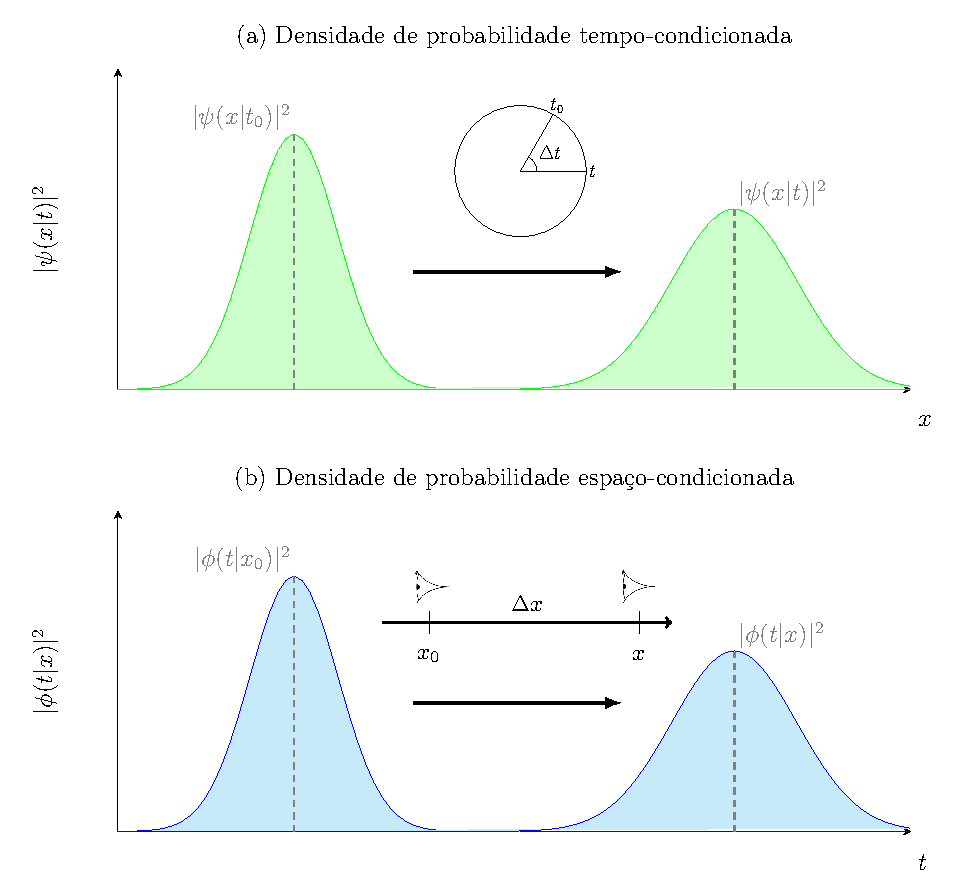
\includegraphics[width=15cm]{anexos/final_sketch_pt.pdf}
    \caption{Os dois sistemas descrevem diferentes situações físicas e têm diferentes propósitos experimentais; enquanto a densidade de probabilidade da mecânica quântica de Schrödinger (a) representada por $|\psi(x|t)|^2$ descreve uma situação em que medimos a posição de uma partícula dado um instante de tempo $t$, na teoria STS (b) representado por $|\pmb{\phi}(t|x)|^2$ medimos o tempo de chegada de uma partícula dada uma posição $x$ no espaço.}
    \label{fig:timevsspace}
\end{figure}


À primeira vista, pode-se pensar que a extensão STS não é projetada para responder ao problema tradicional TOA: Dada uma partícula com uma função de onda de momentos positivos em $t_0$, $\psi(x|t_0)$, restrita à uma região $x<x^* $, quando essa partícula chega na posição $x^*$? Seguindo a interpretação acima, assim como a equação de Schrödinger fornece translações temporais de uma função de onda previamente conhecida $\psi(x|t_0)$, a equação de Schrödinger EC~(\ref{Schro2T}) descreve translações espaciais de uma função de onda EC $\pmb{\phi}(t|x_0)$ que também deve ser conhecida. No entanto, se $\psi(x|t)$ e $\pmb{\phi}(t|x)$ compartilham informações comuns sobre outros observáveis, por exemplo, energia e/ou momento, $\psi(x|t_0)$ pode ajudar a descobrir $\pmb{\phi}(t|x_0)$ e vice-versa.

% Devido à discussão acima e conforme mencionado no início desta seção, devemos saber (i) se $\phi(t|x)$ da extensão STS (se estiver correta) fornece informações complementares a MQ ou (ii) se alguém pode obter $\phi(t|x)$ de $\psi(x|t)$ sem usar a extensão STS. Para analisar esta questão, vamos supor que assim como uma partícula tem um estado bem definido $\psi(x|t)$ para todo o tempo, ela também tem um estado $\phi(t|x)$ para cada posição. No cenário (ii), $\phi(t|x)$ forneceria informações redundantes e poderia ser uma das distribuições TOA ideais existentes. Além disso, $\phi(t|x_0)$ e $\phi(t|x)$ obtidos de $\psi(x|t)$ poderiam ser usados para testar se a equação SC Schrödinger~(\ref{ Schro2T}) está realmente correto. Por outro lado, se $\phi(t|x)$ fornece informações adicionais, $\phi(t|x)$ pode ser obtido através da equação de Schrödinger EC com ou sem a ajuda de $\psi(x|t)$. No último caso, duas condições iniciais, $\psi(x|t_0)$ e $\phi(t|x_0)$, devem ser conhecidas para que se possa prever através das Eqs.~(\ref{Schro2}) e~( \ref{Schro2T}) todas as realizações experimentais possíveis em um determinado sistema físico.


 % A dificuldade em obter uma distribuição TOA ideal de $\psi(x|t)$ para uma posição arbitrária $x$, que eventualmente pode ser identificada como $|\phi(t|x)|^2$, é notável visto a falta de consenso e através dos muitos problemas dos numerosos modelos que existem na literatura. Por exemplo, o TOA ideal dado pelo fluxo quântico requer a mecânica Bohmiana para sua interpretação adequada, visto que o mesmo pode ser negativo e nem sempre pode ser descrito por um POVM (nome atribuído a uma medida de valor de operador positivo). Um outro indício de que não é possível obter $\phi(t|x)$ (ou um TOA ideal em $x$) apenas a partir de $\psi(x|t)$ é que não podemos conhecer uma determinada distribuição condicional ${ \mathcal P}(a|b)$ apenas conhecendo ${\mathcal P}(b|a)$.

%Pode-se ver facilmente que para algumas posições, $x^*$, o estado $\phi(t|x^*)$ pode ser obtido de $\psi(x|t)$. Em particular, se um pacote de ondas inicialmente restrito à região $x<0$ viaja para a esquerda, devemos ter $\phi(t|x^*>0)=0$ já que a partícula nunca chega a $x=x^* $. Porém, para qualquer posição $x$, revela-se a dificuldade em obter uma distribuição TOA ideal de $\psi(x|t)$, que eventualmente pode ser identificada como $|\phi(t|x)|^2$ na falta de consenso e nos problemas dos numerosos modelos disputados na literatura. Por exemplo, a abordagem usando a probabilidade atual $J(x,t)$ considera o raciocínio semiclássico. Aqui se argumenta, por exemplo, que se uma partícula livre com $\psi(x|t_0)$ restrita à região $x<0$ e $J(x,t)>0$, a integral de $|\psi( x|t>t_0)|^2$ em $x<0$ é a probabilidade da partícula não sair desta região no intervalo de tempo $[t_0,t]$. Observe que esta conclusão não é totalmente consistente com QM, onde a partícula não tem uma posição bem definida. A extensão STS lida com essa indeterminação com uma abordagem puramente quântica, introduzindo um estado quântico para cada posição. Outra indicação de que não é possível obter $\phi(t|x)$ apenas de $\psi(x|t)$ é que não podemos conhecer uma certa distribuição condicional ${\mathcal P}(a|b)$ apenas conhecendo ${\mathcal P}(b|a)$ e vice-versa.



%Observamos algumas dificuldades de obter $\phi(t|x)$ a partir de $\psi(x|t)$ enfatizando suas distribuições de probabilidade no tempo e no espaço, respectivamente. No entanto, assim como $\psi(x|t)$, se $\phi(t|x)$ é um estado quântico adicional do sistema, ele também deve determinar as amplitudes de probabilidade de qualquer observável da partícula, como seu energia e impulso. Com isso em mente, vamos agora investigar a extensão STS considerando-a como uma teoria complementar a MQ e usando as bases de energia e quantidade de movimento. Desta forma, observe que se $\psi(x|t)$ e $\phi(t|x)$ compartilham a mesma informação sobre energia e momento, $\psi(x|t)$ pode ajudar a descobrir $ \phi(t|x)$ e vice-versa.

% Por outro lado, tal qual $\psi(x|t)$, que descreve observáveis em um determinado momento, se $\phi(t|x)$ é um estado quântico adicional da partícula, ele também deve determinar amplitudes de probabilidade ( agora em uma determinada posição) associado aos observáveis da partícula. Com isso em mente, vamos agora investigar a extensão STS usando as bases de energia e momento. Observe que se $\psi(x|t)$ e $\phi(t|x)$ compartilham informações comuns sobre energia e/ou momento, $\psi(x|t)$ pode ajudar a descobrir $\phi( t|x)$ e vice-versa.

Com a discussão acima em mente, para buscar uma relação entre $|\psi(t)\rangle$ e $|\pmb{\phi}(x)\rangle$, devemos representá-los na mesma base. Precisamos decompor $|\psi(t)\rangle$ nos autoestados de momento se quisermos compará-lo com a Eq.~(\ref{SolTL}). Sendo assim,
\begin{equation}\label{SolXP}
|\psi(t)\rangle=\int_{-\infty}^{\infty} dP ~ {\tilde \psi}(P|t) |P\rangle_t,
\end{equation}
onde ${_t\langle} x|P\rangle_t=1/\sqrt{2\pi \hbar}\exp{iPx/\hbar}$. Observe que
$|{\tilde \psi}(P|t)|^2$ --- a densidade de probabilidade de medir a partícula com $P$, dado que a observação acontece em $t$ --- é independente do tempo apenas para a situação de partícula livre, onde
\begin{equation}\label{SolXP2}
{\tilde \psi}(P|t)={\tilde \psi}(P)~e^{-i P^2t/(2m\hbar)}.
\end{equation}
Por outro lado, para comparar $|\phi(x)\rangle$ com a Eq.~(\ref{SolXL}), deve-se representá-lo nos autoestados de energia, ou seja,
\begin{equation}\label{SolTE}
|{\pmb \phi}(x)\rangle=\int_{-\infty}^{\infty} dE ~ {\bar {\pmb\phi}}(E|x) |E\rangle_x,
\end{equation}
onde ${_x\langle} t|E\rangle_x=1/\sqrt{2\pi \hbar} \exp{-iEt/\hbar}$. Ressaltamos que ${\bar{\pmb{\phi}}}(E|x)$ é um vetor de duas componentes, ${\bar{{\phi}}}^\pm(E|x)$, e $|{\bar{\pmb{\phi}}} (E|x)|^2={\bar{\pmb{\phi}}}^\dagger(E|x) {\bar{\pmb{\phi}}}(E|x)$ é a densidade de probabilidade de medir a partícula com $E$, dado que a observação acontece em $x$. Para a situação de partícula livre~\cite{Dias},
\begin{equation}\label{SolTE2}
{\bar \phi}^{\pm}(E|x)={\bar \phi}^{\pm}(E)~e^{\pm i \sqrt{2mE} x/\hbar}.
\end{equation}






No intuito de relacionar $|\psi(t)\rangle$ e $|\pmb{\phi}(x)\rangle$ usando a base de momento [Eqs.~(\ref{expansionT}) e~(\ref{SolXP})], vamos comparar as amplitudes de probabilidade ${\tilde \phi}(P_b|x)={\langle} \pmb{P}_b (x)|\pmb{\phi}(x)\rangle$ da Eq.~(\ref{phiP}) e ${\tilde \psi}(P|t)={_t\langle} P|\psi(x)\rangle$. Em geral, a impossibilidade de conectar essas duas funções de onda é porque enquanto $|{\tilde \psi} (P|t)|^2$ prevê dados experimentais sobre o momento da partícula coletados em um instante fixo $t$, independentemente da posição observada, $ |{\tilde \phi}(P_b|x)|^2$ prevê dados sobre o momento coletados em uma posição fixa $x$, independentemente do tempo observado. Claramente, eles representam diferentes distribuições de probabilidade. Por exemplo, se uma função de onda $\psi(x|t)$ não pode atravessar uma barreira de potencial, a partícula nunca atinge uma certa posição $x^*$ no lado da transmissão. Nessa situação, ${\tilde \phi}(P_\pm|x^*)$ da Eq.~(\ref{phiPFree}) é zero para todo $P$, enquanto ${\tilde \psi }(P,t) \neq 0$. Vemos que para vincular as funções de onda de momento, nós enfrentamos o mesmo problema de relacionar $\psi(x|t)$ e $\pmb{\phi}(t|x)$: enquanto $|\psi(t)\rangle$ descreve observáveis em um determinado momento, $|\pmb{\phi}(x)\rangle$ descreve os mesmos observáveis, mas em uma determinada posição.





%Vamos analisar a situação específica em que uma partícula livre sempre chega a um determinado ponto $x^*$, ou seja, $\langle \phi(x^*)|\phi(x^*)\rangle=1$. Nesse caso, todo o pacote de ondas $\psi(x|t)$ passa por $x^*$, significando que todas as amplitudes de Fourier (momento) contribuem para a chegada em $x^*$. Conseqüentemente, todos os momentos da distribuição independente do tempo $|{\tilde \psi}(P|t)|^2=|{\tilde \psi}(P)|^2$ podem ser medidos se o detector estiver localizado em $x^*$. Neste cenário, esperamos que ${\tilde \phi}(P|x^*)$ --- a probabilidade da partícula ter momento $P$, dado que ela é observada em $x^*$, independentemente do tempo que chega --- é igual a $|{\tilde \psi}(P)|^2$. Finalmente, se assumirmos que suas fases também são as mesmas, ou seja, ${\tilde \psi}(P)={\tilde \phi}(P)$, $\rho(t|x)$, obtemos a distribuição que Kijowski propôs axiomaticamente usando MQ ortodoxa. Portanto, configurações experimentais que medem a distribuição de Kijowski também medem $\rho(t|x)$ para a situação de partícula livre.


%Embora não possamos relacionar $\phi(t|x)$ diretamente com $\psi(x|t)$ para situações mais gerais, podemos comparar modelos que usam $\psi(x|t)$ para obter o TOA ideal para uma partícula atravessando uma região de potencial com as previsões da extensão STS para este mesmo problema. Na próxima seção, resolveremos a evolução espacial(\ref{rhoX}) para um potencial arbitrário independente do tempo provendo assim essa comparação tanto para o regime de tunelamento quanto para o de partícula livre, isto é, quando o potencial for nulo.



Vamos focar a discussão acima na situação mais simples possível, uma partícula livre com momentos positivos $P^+=P>0$ que sempre chega a um determinado ponto $x^*$, ou seja, $\langle \pmb{\phi}(x^ *)|\pmb{\phi}(x^*)\rangle=1$. Essa situação é descrita pela solução~(\ref{SolTL}) com ${\tilde \phi}^-(P)=0$. ~À medida que todo o pacote de onda $\psi(x|t)$ passa por $x^*$, todos os momentos possíveis da distribuição independente do tempo $|{\tilde \psi}(P|t)|^2=| {\tilde \psi}(P)|^2$ podem ser medidos se um detector estiver em $x^*$. Nesse cenário, pode-se esperar que $|{\tilde \psi}(P)|^2$ seja igual a $|{\tilde \phi}(P_+|x^*)|^2=|{\tilde \phi}^+(P)|^2$ (a probabilidade da partícula ter momento $P$, dado que é observada em $x^*$, independentemente do instante em que chega). Se também assumirmos que suas fases são as mesmas, ou seja, ${\tilde \phi}^+(P)={\tilde \psi}(P)$ (o que não é uma suposição trivial), $\rho(t| x)$ da Eq.~(\ref{pd}) torna-se a distribuição de Kijowski, conforme considerado na Ref.~\cite{Dias} sem maiores justificativas. No entanto, vale notar que mesmo que ${\tilde \phi}(P)={\tilde \psi}^+(P)$, $\pmb{\phi}(t|x)$ ainda representa informação complementar à MQ pois a equação de Schrödinger EC~(\ref{Schro2T}) ainda é necessária para obter a solução~(\ref{SolTL}).

Da discussão desta seção, concluímos que, se a extensão STS estiver correta, sua informação não está totalmente incorporada no estado \textit{intrínseco} da partícula $|\psi(t)\rangle$. Por outro lado, como é o objetivo de qualquer modelo de TOA ideal, esperamos que as previsões de $|\pmb{\phi}(t|x)|^2$ possam ser confirmadas tomando alguns limites de medidas ideais, onde detectores bem projetados e/ou relógios acoplados à partícula registram seu TOA. Neste caso, a informação de $|\pmb{\phi}(t|x)|^2$ não está no estado de "medição livre"\text{ }da partícula ($\psi(x|t)$), mas, por exemplo, no estado do relógio ($\rho_C \in {\mathcal H}_t$). Outra forma de recuperar $|\pmb{\phi}(t|x)|^2$ (se ${\tilde \phi}^\pm(P)={\tilde \psi}(\pm P)$) a partir de um modelo operacional é através do cálculo da densidade de probabilidade temporal de detectar o primeiro fóton emitido quando um átomo de dois níveis entra em uma região iluminada por um laser~\cite{Damborenea}. Usando as técnicas de salto quântico e a ``normalização de operador''~\cite{Brunetti}, esta densidade de probabilidade torna-se a distribuição de Kijowski no limite de campo forte e decaimento rápido~\cite{Heger}.


% Os efeitos da fase serão investigados em outro lugar. Observe que eles podem ter o mesmo Phi se a diferença de fases for tal que. Se as fases são de fato diferentes, temos que obtê-la de outra forma, ou precisamos de uma condição inicial adicional $\phi\left(t \mid x^*\right)$, phi( $\left.\mathrm{ P}, \mathrm{x} 0\right)$ para obter $\operatorname{phi}(\mathrm{P}-\mathrm{x})$ e com isso phi $(\mathrm{t}-\mathrm{ x})$.





%Um exemplo da diferença discutida acima pode ser visto em uma partícula com o estado inicial da MQ dado por $\left|\psi\left(t_0\right)\right\rangle=\left|P_1\right\rangle_t+\left| P_2\right\rangle_t$, onde $P_2>P_1>0$, chegando pela esquerda em uma barreira de potencial. Suponha que apenas $\left|P_2\right\rangle_t$ possa passar pela barreira de potencial definida na região $0 \leq x \leq a$. Depois de um tempo, o estado da MQ envolve uma combinação linear de estados provenientes da reflexão de $\left|P_1\right\rangle_t$ e $\left|P_2\right\rangle_t$ e da transmissão de  $\left|P_2\right\rangle_t$. Por outro lado, como o estado na extensão STS é definido em uma determinada posição, o estado da partícula em $x>a$ deve ser $\left|\phi^{+}(x)\right\rangle= \alpha\left|P_2\right\rangle_x$, onde $1-|\alpha|^2$ é a probabilidade de que a partícula nunca chegue a $x>a$ por causa da reflexão de $\left|P_2\right\rangle_t $. O fator $\alpha$ deve ser quantificado pela equação de Schrödinger EC (\ref{Schro2T}).


\chapter{Soluções para $V=V(x)$ e o TOA de uma partícula atravessando uma barreira de potencial}
\label{chap:cap4}

Neste capítulo iremos resolver a equação de Schrödinger EC para um potencial arbitrário independente do tempo. Em seguida, aplicaremos esta solução para prever o TOA de uma partícula atravessando uma barreira de potencial quadrada, assumindo que ${\tilde \phi}^+(P)={\tilde \psi}(P)$ para uma partícula livre incidindo com momento $P>0$. Também compararemos nossos resultados com uma generalização da distribuição de Kijowski~\cite{Delgado,Leon,Baute2} e discutiremos as consequências de assumir ${\tilde \phi}^+(P)={\tilde \psi}(P)$.

\section{Solução geral da equação de Schrödinger EC para $V = V(x)$}
\label{sec:solVarb}

A equação de Schrödinger EC~(\ref{SchroT}) para um potencial arbitrário independente do tempo $V=V(x)$ torna-se mais simples usando a representação de energia, $\{|E\rangle_x\}$.
 Substituindo a Eq.~(\ref{SolTE}) na equação de Schrödinger EC~(\ref{SchroT}), nos leva a
\begin{eqnarray}\label{sol1}
&&\int_{-\infty}^{\infty} dE~{\sigma}_{z}~{\bar{\pmb{\phi}}}(E|x) ~\sqrt{2m\big[{\hat {\mathbbm H}}-V(x){\hat {\mathbb I}}\big]}~|E\rangle_x\nonumber\\
&=&-\int_{-\infty}^{\infty} dE~i\hbar\frac{d {\bar{\pmb{\phi}}}(E|x)}{dx}~|E\rangle_x.
\end{eqnarray}
Ao explandir o operador $\sqrt{{\hat {\mathbbm H}- V(x){\hat {\mathbbm I}}}}$, para $V(x)\neq 0$, em séries de potência, nós obtemos
\begin{eqnarray}
\sqrt{{\hat {\mathbbm H}}-V(x){\hat {\mathbbm I}}}=\sum_{n=0}^{\infty} {\frac{1}{2}\choose n} i^{1-2n} [V(x)]^{\frac{1}{2}-n}~{\hat {\mathbb H}}^n,
\end{eqnarray}
que aplicado em $|E\rangle_x$ nos leva a
\begin{eqnarray}
&&\sum_{n=0}^{\infty} {\frac{1}{2}\choose n} i^{1-2n} [V(x)]^{1/2-n}~{\hat {\mathbbm H}}^n|E\rangle_x\nonumber\\
&=&\sum_{n=0}^{\infty} {\frac{1}{2}\choose n} i^{1-2n} [V(x)]^{1/2-n}E^n|E\rangle_x\nonumber\\
&=&\sqrt{E-V(x)}~|E\rangle_x.
\end{eqnarray}
Substituindo essa equação de volta na Eq.~(\ref{sol1}), e projetando a expressão resultante em $|E'\rangle_x$, obtemos uma equação diferencial para $\bar{\pmb{\phi}}(E'|x)$ dada por
\begin{eqnarray}
{\sigma}_z\sqrt{2m\big[E'-V(x)\big]}~{\bar{\pmb{\phi}}}(E'|x)=-i\frac{d}{dx}{\bar{\pmb{\phi}}}(E'|x),
\end{eqnarray}
cuja solução de cada componente é tal que
\begin{equation}\label{SolE}
{\bar \phi}^\pm(E|x)=\frac{{\bar \phi}^\pm(E|x_0)}{\sqrt{2\pi \hbar}}e^{{\pm}i \bigintssss_{x_0}^x dx'\sqrt{2m [E-V(x') ]}/\hbar},
\end{equation}
onde substituímos $E'$ por $E$. Substituindo a Eq.~(\ref{SolE}) em $|\pmb{\phi}(x)\rangle$ da Eq.~(\ref{SolTE}), e então projetando a expressão resultante em $|t\rangle_x$, obtemos
\begin{eqnarray}\label{SolTX}
\phi^\pm(t|x)= \int_{-\infty}^{\infty}dE~\frac{{\bar \phi}^\pm(E|x_0)}{\sqrt{2\pi \hbar}}~e^{{\pm}i \bigintssss_{x_0}^x dx'\sqrt{2m [E-V(x') ]}/\hbar-iEt/\hbar}.
\end{eqnarray}
Essa é a solução geral para a amplitude de probabilidade do TOA ideal na posição $x$ de uma partícula sob a ação de $V=V(x)$. Tomando $V(x)=0$, impondo a normalização no tempo, e mudando a variável de integração para $P_\pm$, recuperamos a solução de partícula livre cuja amplitude de probabilidade é dada pela Eq.~(\ref{SolTL}).


Vale notar a semelhança entre a Eq.~(\ref{SolTX}), válida para $V=V(x)$, e a solução da equação de Schrödinger para potenciais dependentes exclusivamente do tempo, $V=V (t)$, que é dado por
\begin{equation}\label{SolXT}
\psi(x|t)=\int_{-\infty}^{\infty} dP \frac{{\tilde \psi}(P|t_0)}{\sqrt{2\pi \hbar}} e^{-i\bigintssss_{t_0}^t dt'[{P^2}/(2m)+V(t')]/\hbar +iPx/\hbar}.
\end{equation}
Aqui observamos que se pode ir de uma solução para a outra através da transformação $(t,P,H(t)) \rightarrow (x,E,\pm P(x))$, com $H(t)$ e $P(x)$ dados pelas expressões clássicas das Eqs.~(\ref{ruleX}) e~(\ref{ruleP}), respectivamente. Essa simetria fica ainda mais evidente ao identificar a ação clássica $S$ na Eq.~(\ref{SolTX}), para $V=V(x)$, e na Eq.~(\ref{SolXT}), para $V=V(t)$, o que nos permite reescrevê-las como
\begin{equation}
\phi^\pm(t|x)=\frac{1}{\sqrt{2\pi \hbar}}\int_{-\infty}^{\infty} dE~ {\bar \phi}^\pm(E|x_0)~e^{-iS(E,x)/\hbar}
\end{equation}
e também
\begin{equation}
\psi(x|t)=\frac{1}{\sqrt{2\pi \hbar}}\int_{-\infty}^{\infty}d{P}~ {\tilde \psi}(P|t_0)~e^{-iS(P,t)/\hbar}.
\end{equation}

Usando a solução da Eq.~(\ref{SolTX}), na próxima seção, vamos calcular a distribuição TOA de uma partícula atravessando uma barreira de potencial.


\section{Comparando as previsões do STS com uma generalização da distribuição de Kijowski}
\label{sec:comparandosol}

Apliquemos a solução~(\ref{SolTX}) à uma partícula livre preparada muito à esquerda da origem e detectada após cruzar uma barreira quadrada de altura $V_0$, largura $L$ e localizada no intervalo $0 < x < L$. A partícula inicialmente tem um estado na MQ usual dado por um pacote de onda gaussiano centrado em $x_i$ ($\hbar=1$),
\begin{equation}\label{initialX}
\psi(x|t_i)=\frac{1}{(2\pi \delta^2)^{1/4}}e^{- \left[(x-x_i)/(2\delta)-iP_i\delta\right]^2- P_i^2\delta^2 },
\end{equation}
onde $\psi(x|t_i)={_t\langle}x|\psi(t_i)\rangle$. Aqui $x_i$, $P_i$ e $\delta$ assumirão valores tais que o pacote esteja à esquerda da origem e tenha apenas momentos positivos. Nesse contexto, para calcular o TOA no lado da transmissão usando a interpretação da equação de Schrödinger EC dada na seção anterior, devemos aplicar a solução~(\ref{SolTX}) à uma amplitude de probabilidade inicial do TOA, $\pmb{\phi}(t|x_0)$, com $x_0$ localizado no lado esquerdo da barreira, $x_i < x_0 \leq 0$. Consideramos $\psi(x_0|t_i)\approx 0$, significando que no tempo $t_i$, a partícula não chegou a $x_0$. Conforme discutido na Sec.~(3.2), uma vez que a partícula viaja livremente no lado esquerdo da barreira e sempre passa pelo ponto $x_0$, vamos assumir que $|\pmb{\phi}(t|x_0)|^2$ é a distribuição de Kijowski~(\ref{pd}), ou seja, ${\tilde \phi}^+(P)={\tilde \psi} (P)$, onde ${\tilde \psi}(P)$ é a função de onda de momento de $\psi(x|t_i)$,
\begin{equation}\label{initialXP}
{\tilde \psi(P)}=\left(\frac{2\delta^2}{\pi}\right)^{1/4}e^{-\delta^2 (P-P_i)^2 -iPx_i}.
\end{equation}






Note que na formulação atual da extensão STS, $\phi^+(t|x)$ e $\phi^-(t|x)$ obedecem a duas equações independentes. Portanto, como estamos interessados no TOA da partícula na região transmitida, onde existem apenas momentos positivos, vamos nos concentrar exclusivamente em $\phi^+(t|x)$. Voltaremos a discutir essa independência entre $\phi^+(t|x)$ e $\phi^-(t|x)$ no final desta seção. Usando as Eqs.~(\ref{SolTL}) e~(\ref{initialXP}) nessas circunstâncias, a condição ``inicial'' em $x_0$ da função de onda EC torna-se
\begin{eqnarray} \label{initialT}
\phi^+(t|x_0)= 
\int_0^{\infty}dP~{\tilde \psi}(P)\sqrt{\frac{|P|}{2\pi
m\hbar}}~e^{iPx_0/\hbar-iP^2t/(2m\hbar)},\nonumber\\
\end{eqnarray}
onde $P=\sqrt{2mE}$. Para aplicar a solução EC~(\ref{SolTX}) à $\phi^+(t|x_0)$, temos que descobrir ${{\bar \phi}^+}(E|x_0)$ para essa condição ``inicial'' particular. Considerando $x_0=0$, Eq.~(\ref{SolTX}) em $x=x_0$, onde $V(x_0)=0$, se reduz a
\begin{eqnarray}\label{SolTX2}
\phi^+(t|x_0)=\frac{1}{\sqrt{2\pi \hbar}}
\int_{-\infty}^{\infty}dE~{\bar \phi}^+(E|x_0)e^{-iEt/{\hbar}}.
\end{eqnarray}
Mudando a variável de integração $P$ na Eq.~(\ref{initialT}) para $E$, e comparando a expressão resultante com a Eq.~(\ref{SolTX2}), identificamos
\begin{eqnarray}\label{Const}
{\bar \phi}^+(E|x_0)=\Theta(E)\left(\frac{m}{2E}\right)^{1/4} {\tilde \psi}(\sqrt{2mE}),
\end{eqnarray}
onde $\Theta(E)$ é a função degrau de Heaviside. Finalmente, substituindo a Eq.~(\ref{Const}) na função de onda EC~(\ref{SolTX}) para a barreira de potencial quadrada, e calculando em $x>L$, obtemos
\begin{eqnarray}\label{SolTBarrier}
\phi^+(t|x)&=&\frac{1}{\sqrt{2\pi \hbar}}
\int_{-\infty}^{\infty}dE  ~\left(\frac{m}{2E}\right)^{1/4} {\tilde \psi}(\sqrt{2mE})\nonumber\\ &\times& e^{i\sqrt{ 2m \left( E - V_0 \right)} L/\hbar + i\sqrt{ 2m E} (x-L)/\hbar -iEt/\hbar}.\nonumber\\
\end{eqnarray}
Esta solução nos dá a amplitude de probabilidade temporal da partícula chegar em $x > L$.



O fato de considerarmos ${\tilde \phi}^+(P)={\tilde \psi}(P)$ para a partícula incidente, nos permite calcular o tempo de chegada após a barreira usando a extensão STS de outra forma. Como a partícula transmitida sempre passa por $x>L$ e ela também está livre nessa região, podemos considerar também ${\tilde \phi}^+_T(P)={\tilde \psi}_{T}( P)$, onde ${\tilde \phi}^+_T(P)$ é o coeficiente da Eq.~(\ref{SolTL}) para $x>L$ e ${\tilde \psi}_T(P )=T(P){\tilde \psi}(P)$ é a função de onda de momento do pacote transmitido, com
\begin{equation}\label{Trans}
    T(P) = \frac{4 P P' e^{-i(P - P')L/\hbar}}{\left(P + P' \right)^2 - e^{2 iP'L/\hbar} \left(P - P' \right)^2}
\end{equation}
sendo o coeficiente de transmissão e $P'=\sqrt{P^2-2mV_0}$. Substituindo ${\tilde \psi}_{T}(P)$ na Eq.~(\ref{pd}), com ${\tilde \phi}^-(P)=0$, $\rho(t| x)$ torna-se
\begin{eqnarray}\label{KijoG}
    &&\Pi_{K}^{N} (t|x) = \frac{1}{\int_0^\infty dP |T(P){\tilde \psi}(P)|^2}
    \nonumber\\
    &&\times\frac{\hbar}{2 \pi m \hbar} \left| \int_0^\infty dP~T(P){\tilde \psi}(P) e^{-i \hbar P^2 t / (2m\hbar) + i \hbar P (x-L)/\hbar}  \right|^2.\nonumber\\
\end{eqnarray}
Note que aqui usamos que a probabilidade da partícula chegar em $x$, independentemente do tempo (${\langle \pmb{\phi}(x)|\pmb{\phi}(x) \rangle}$) é igual a probabilidade da partícula ser transmitida ($( \int_0^\infty dP |T(P){\tilde \psi}(P)|^2)$. A equação~(\ref{KijoG}) é a distribuição Kijowski normalizada para o pacote transmitido. Esta equação nos fornece a densidade de probabilidade para o TOA em $x$, dado que a partícula foi transmitida através da barreira de potencial. Essa abordagem já foi considerada anteriormente na Ref.~\cite{Ricardo}. Nesse trabalho, é mostrado que para um experimento eletromagnético que simula o tunelamento quântico~ \cite{Ranfa}, o tempo médio de percurso obtido via Eq.~(\ref{KijoG}) concorda melhor com os dados experimentais do que os modelos Büttiker-Landauer e o \textit{phase-time}.




Vale ressaltar que a Eq.~(\ref{KijoG}) foi obtida por diferentes métodos usando a MQ usual~\cite{Delgado,Leon,Baute2}. Em particular, ela surge do mesmo modelo operacional discutido no final do capítulo 3, que calcula o tempo de detecção do primeiro fóton emitido quando um átomo de dois níveis entra em uma região iluminada por um laser. Nessa situação, quando uma barreira de potencial quadrada está presente, e tomamos os limites de um campo de laser forte e decaimento rápido, a distribuição do TOA em $x>L$ torna-se Eq.~(\ref{KijoG}) para as partículas transmitidas~\cite{ Heger2}. 


Abaixo comparamos as distribuições do TOA das Eqs.~(\ref{SolTBarrier}) e~(\ref{KijoG}) e investigamos se as suposições ${\tilde \phi}^+(P)={\tilde \psi} (P)$ e ${\tilde \phi}^+_T(P)={\tilde \psi}_{T}(P)$ levam a inconsistências na extensão STS.
\begin{figure}[H]
    \centering
    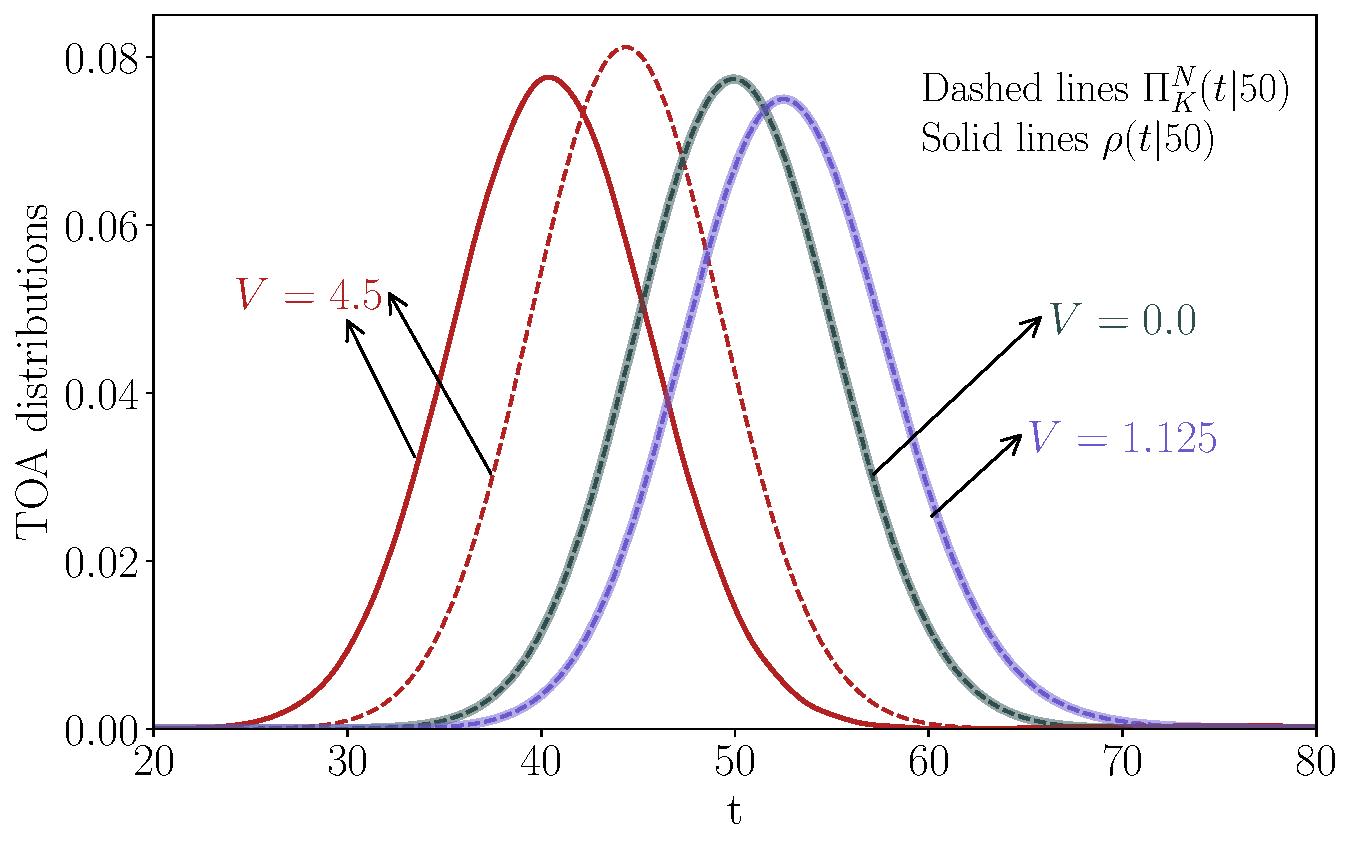
\includegraphics[width=14cm]{anexos/paper.pdf}
    \caption{Distribuições de probabilidade para o tempo de chegada das partículas transmitidas em $x=50$. O pacote de onda inicial, $\psi(x,t_i)$, possui $P_0=2$, $\delta=10$, $x_0=-50$ e $m=1$. A largura da barreira é $L = 10$. A linha contínua (trecejada) ilustra a previsão de $\rho(t|x)$ ($\Pi_K^N(t|x)$). Note que essas distribuições discordam no regime de tunelamento.}
    \label{fig:paper}
\end{figure}


Nós plotamos a distribuição de probabilidade do TOA na figura acima usando os mesmos parâmetros físicos da Ref.~\cite{Leon}. Essa referência obtém a Eq.~(\ref{KijoG}) transformando canonicamente o TOA da partícula livre. No gráfico, a largura da barreira é $L=10$, o detector está em $x=50$, e os parâmetros do pacote de onda inicial~(\ref{initialX}) são $x_i=-50$, $P_0=2$, $\delta= 10$ e $m=1$. As curvas sólidas e tracejadas mostram a distribuição do TOA em $x=50$ usando as Eqs.~(\ref{SolTBarrier}) e~(\ref{KijoG}), respectivamente, para $V_0=0 $, $V_0=1.125$ e $V_0=4.5$. Este último representa o regime de tunelamento. Observe que o TOA clássico de uma partícula livre com velocidade $P_0/m=2$ é $50$, já que o comprimento total do caminho da partícula é $100 $ unidades.



Ao inspecionar a Fig.~\ref{fig:paper} primeiro observamos que em comparação com a situação de transmissão livre, $V_0=0$, tanto as curvas sólidas quanto as tracejadas ilustram um atraso do TOA para $V_0<E_0=P_0^2/(2m)$ e avanço para $V_0>E_0$. Além disso, embora as expressões~(\ref{SolTBarrier}) e~(\ref{KijoG}) sejam matematicamente diferentes, elas concordam muito bem para $V_0<E_0$. No entanto, no regime de tunelamento, vemos que a Eq.~(\ref{SolTBarrier}) antecipa o tempo de chegada em relação à previsão da Eq.~(\ref{KijoG}). Essa discordância mostra que se as relações ${\tilde \phi}^+(P)={\tilde \psi}(P)$ e ${\tilde \phi}^+_T(P)={\tilde \psi }_{T}(P)$ estão corretos, a extensão STS deve ser reformulada de alguma forma. No entanto, se ${\tilde \phi}^+(P) \neq {\tilde \psi}(P)$ e/ou ${\tilde \phi}^+_T(P) \neq {\tilde \psi }_{T}(P)$, a solução~(\ref{SolTBarrier}) ainda pode estar correta.



Voltando ao que discutimos anteriormente, o conflito acima pode vir do fato de que $\phi^+(t|x)$ e $\phi^-(t|x)$ são tratados independentemente na Eq. ~(\ref{SolTBarrier}). Observe que $\phi^+(t|x)$ e $\phi^-(t|x)$ são desacoplados tanto na equação de Schrodinger EC~(\ref{Schro2T}) quanto na distribuição de probabilidade temporal~(\ref {rhoT}). Esse tratamento negligencia, por exemplo, a interferência entre momentos positivos e negativos. Essa independência também ocorre na distribuição Kijowski e foi originalmente criticada por Leavens \cite{LeavensR}. Vale ressaltar que usando a técnica de normalização de operador mencionada no Cap.~\ref{chap:cap2} para um potencial absorvedor fraco e estreito (definindo a região iluminada), Ref.~\cite{Heger2} generaliza a distribuição Kijowski levando em conta a interferência entre momentos positivos e negativos. Com essa discussão em mente, mudanças fisicamente plausíveis na extensão STS para acoplar as funções de onda EC de momentos positivos e negativos estão sendo investigadas para um próximo trabalho. 







  \chapter{Conclusão e considerações finais}
\label{chap:conclusao}


Nesta dissertação, revisitamos a ideia de que o problema do tempo na mecânica quântica está enraizado na objeção de Pauli, que questiona a relação de comutação entre operadores de tempo e energia. Essa objeção impulsionou o desenvolvimento de diversas abordagens para incorporar um operador tempo na mecânica quântica. No entanto, todas elas exigem o abandono da hermiticidade ou da relação de comutação com hamiltoniano. Além disso, o problema do tempo transcende a não existência de um operador auto adjunto para o tempo, pois envolve também o conceito de tempo de chegada, que não pode ser adequadamente definido no âmbito da mecânica quântica convencional.


Com esses fatos em mente, exploramos a extensão STS e as previsões de seus estados "espaço-condicionais"\text{ }(EC) para potenciais arbitrários, comparando-as com as previsões "tempo-condicionais"\text{ }da MQ usual. Vimos no Cap. \ref{chap:cap2} que o estado quântico (EC) $|\pmb{\phi}(x)\rangle$ definido em cada ponto do espaço é intrínseco à partícula, e quando expandido na base tempo, seus coeficientes representam a amplitude de probabilidade de TOA ideal na posição $x$. Ao investigarmos no Cap. \ref{chap:cap3} o comportamento da equação de autovalor do momento para um potencial arbitrário, constatamos que para potenciais dependentes do espaço, estados com momento bem definido dependem da posição, da mesma forma que estados com energia bem definida na MQ usual dependem do tempo para potenciais dependentes do tempo.


Buscamos então nesse trabalho apresentar uma interpretação clara para a equação de Schrödinger EC. Trabalhamos com a ideia que dada uma função de onda EC "inicial"\text{ }$\pmb{\phi}(t|x_0)$, a solução $\pmb{\phi}(t|x)$ é a amplitude de probabilidade da partícula chegar no instante $t$, dado que iremos agora detectar a mesma em uma nova posição $x$. Além disso, tentamos estabelecer uma relação entre os estados TC ($|\psi(t) \rangle$) e EC ($|\pmb{\phi}(x)\rangle$). Para essa comparação utilizamos amplitudes de probabilidade ${\tilde \phi}(P_b|x)$ e ${\tilde \psi}(P|t)$ da base de momento. O problema é que essas duas funções de onda representam diferentes distribuições de probabilidade: enquanto $|{\tilde \psi} (P|t)|^2$ prevê dados experimentais sobre o momento da partícula coletados em um instante fixo $t$, independentemente da posição observada, $ |{\tilde \phi}(P_b|x)|^2$ prevê dados coletados sobre o momento em uma posição fixa $x$, independentemente do tempo observado. A partir disso, ficou claro que se a extensão STS é uma teoria correta, ela deve fornecer informação complementar à MQ. Por fim, ao resolver a Eq. de Schrödinger EC para um potencial arbitrário $V = V(x)$ e aplicar para uma barreira de potencial, pudemos comparar seu comportamento com uma generalização da distribuição de Kijowski. Concluímos que as diferenças observadas entre essas distribuições pode vir do fato da extensão STS negligenciar a interferência entre os momentos positivos e negativos.



Uma perspectiva de mudança da extensão STS fornecida por esse trabalho é através do acoplamento das funções de onda EC $\phi^+ (t|x)$ e $\phi^- (t|x)$, permitindo a interferência entre momentos positivos e negativos. Pretendemos também investigar modelos operacionais do TOA (via a MQ tradicional) que ao assumir algumas idealizações dos equipamentos de medida, relatam previsões de TOA ideal previsto pela extensão STS. Por fim, uma generalização natural da extensão STS é estender suas equações para descrever o TOA em três dimensões e considerar efeitos relativísticos. 














\bookmarksetup{startatroot}% 


% ----------------------------------------------------------
% ELEMENTOS PÓS-TEXTUAIS
% ----------------------------------------------------------
\postextual


% ----------------------------------------------------------
% Referências bibliográficas
% ----------------------------------------------------------
%\bibliographystyle{abntexalfenglish} %caso seja em inglês, retire o comentário desta linha

% \renewcommand{\bibname}{REFER\^ENCIAS}
%\renewcommand{\bibname}{Bibliography}
% \addbibresource{sample.bib}
% \bibliography{mendeley}
\bibliography{references2}

%\newpage
\begin{thebibliography}{0}

\bibitem{1} G. R. Allcock, Ann. Phys. (N.Y.) 53, 253 (1969); 53, 286 (1969); 53, 311 (1969)

\bibitem{2} V. Delgado, J. G. Muga. (1997). Arrival time in quantum mechanics [\textcolor{blue}{arXiv:quant-ph/9704010}]

\bibitem{3} Siddhant D, Markus N. Times of arrival and gauge invariance, June 2021. [\textcolor{blue}{https://doi.org/10.1098/rspa.2021.0101}]

\bibitem{4} C. Leavens, Phys. Rev. A 58, 840 (1998).

\bibitem{5} L. Egusquiza, J. Muga, Andres D. Standard Quantum Mechanical Approach to Times of Arrival. August 2001. [\textcolor{blue}{https://link.springer.com/book/10.1007/978-3-642-03174-8}]

\bibitem{6} Kijowski J. On the time operator in quantum mechanics and the Heisenberg uncertainty relation for energy and time. 1974.  [\textcolor{blue}{doi:10.1016/S0034-4877(74)80004-2}]

\bibitem{7} Kijowski J. Comment on arrival time in quantum mechanics and time of arrival in quantum mechanics. 1999 [\textcolor{blue}{doi:10.1103/PhysRevA.59.897}]

\bibitem{8} J Leon, J Julve, P Pitanga, J Urries. Time of arrival through a quantum barrier. March 1999. [\textcolor{blue}{https://arxiv.org/abs/quant-ph/9903060}]

\bibitem{9} Busch, P. (n.d.). The Time Energy Uncertainty Relation. Lecture Notes in Physics, 73 105. [\textcolor{blue}{doi:10.1007/978-3-540-73473-4-3}] 

\bibitem{10} J., G. D. Introduction to quantum mechanics. Prentice Hall, 2004.

\bibitem{11} Ximenes, Ricardo \& Dias, Eduardo. (2017). Physical and mathematical properties of the space-time-symmetric formalism. [\textcolor{blue}{arXiv:1712.03446v1}]

\bibitem{13} R. Landauer and Th. Martin. Barrier interaction time in tunneling. Reviews of Modern Physics,
66(1):217–228, 1994

\bibitem{14} J. J. Halliwell and J. M. Yearsley. Quantum Arrival Time Formal from Decoherent Histories.
arXiv:0903.1958v2, Mar 2009.


\bibitem{18} V. S. Olkhovsky, E. Recami, and J. Jakiel. Unified time analysis of photon and particle tunnelling.
Physics Reports, 398(3):133–178, August 2004.

\bibitem{20} G. Privitera, G. Salesi, V. S. Olkhovsky, and E. Recami. Tunnelling times : An elementary introduction.
Rivista del Nuovo Cimento, 26(4):1–55, 2003.

\bibitem{28} J. A. Damborenea, I. L. Egusquiza, J. G. Muga, and B. Navarro. Quantum dwell times. arXiv:quantph/0403081v1, (1):1–4, 2004.

\bibitem{31} H. G. Winful. Tunneling time, the Hartman effect, and superluminality: A proposed resolution of an
old paradox. Physics Reports, 436:1–69, December 2006.

\bibitem{Time} J. G. Muga, R. Sala Mayato, I. L. Egusquiza, eds., {\textit Time in Quantum Mechanics}, 2nd ed., Lect. Notes. Phys. 734, Vol. 1 (Springer, Berlin Heidelberg 2008); J.G. Muga, A. Ruschaupt, A. del Campo, eds., {\textit Time in Quantum Mechanics}, Vol. 2, Springer, Berlin Heidelberg (2009).

\bibitem{Aharonov} Y. Aharonov and D. Bohm, Time in the quantum theory and the uncertainty relation for time and energy, Phys. Rev. {\textbf 122}, 1649 (1961).


\bibitem{Galapon} E. A. Galapon, F. Delgado, J. G.Muga, and I. Egusquiza, Transition from discrete to continuous time-of-arrival distribution for a quantum particle, Phys. Rev. A {\textbf 72}, 042107 (2005).

\bibitem{Grot} N. Grot, C. Rovelli, and R. S. Tate, Time of arrival in quantum mechanics, Phys. Rev. A {\textbf 54}, 4676 (1996).


\bibitem{DelMuga} V. Delgado, J.G. Muga, Phys. Rev. A \textbf{56}, 3425 (1997).


\bibitem{All} G.R. Allcock, Ann. Phys. (N.Y.) \textbf{53}, 253 (1969); G.R. Allcock,
Ann. Phys. (N.Y.) \textbf{53},  286 (1969); G.R. Allcock, Ann. Phys.
(N.Y.) 53, 311 (1969).


\bibitem{Baute} A.D. Baute, R. Sala Mayato, J.P. Palao, J.G. Muga, I.L.
Egusquiza, Phys. Rev. A \textbf{61}, 022118 (2000).


\bibitem{Pauli} W. Pauli, General Principles of Quantum Mechanics (Springer, 1980).

\bibitem{Delgado} V. Delgado and J.G. Muga, Arrival time in quantum mechanics, Phys. Rev. A 56, 3425 (1997).


\bibitem{Kijo} J. Kijowski, On the time operator in quantum mechanics and the Heisenberg uncertainty relation for energy and time, Rep. Math. Phys. {\textbf 6}, 361 (1974).


\bibitem{Das} S. Das and W. Struyve, Questioning the adequacy of certain quantum arrival-time distributions, Phys. Rev. A {\textbf 104}, 042214 (2021).


\bibitem{Vona} N. Vona and D. D\"urr, {\textit The role of the probability current for time measurements}, in The Message of Quantum Science: Attempts Towards a Synthesis, edited by P. Blanchard and J. Fr\"ohlich (Springer, 2015) pp. 95-112.

\bibitem{Bracken} A. J. Bracken and G. F. Melloy, J. Phys. A: Math. Gen. {\textbf 27}, 2197 (1994).

\bibitem{Leavens} C. Leavens, On the ``standard'' quantum mechanical approach to times of arrival, Phys. Lett. A {\textbf 303}, 154 (2002).

\bibitem{Das2} S. Das and M. N\"oth, Times of arrival and gauge invariance, Proc. R. Soc. A: Math. Phys. Eng. Sci. {\textbf 477}, 2250 (2021).


\bibitem{Egu} I. Egusquiza, J. Muga, B. Navarro, and A. Ruschhaupt, Comment on: ``On the ``standard'' quantum-mechanical approach to times of arrival'', Phys. Lett. A {\textbf 313}, 498 (2003).


\bibitem{LeavensR} C. Leavens, Reply to Comment on: ``On the ``standard'' quantum-mechanical approach to times of arrival'' [Phys. Lett. A {\textbf 313}, 498 (2003)], Phys. Lett. A {\textbf 345}, 251 (2005).

\bibitem{Miel} B. Mielnik, Found. Phys. \textbf{24}, 1113 (1994).


\bibitem{Allcock} G. R. Allcock, Ann. Phys. {\textbf 53}, 286 (1969).

\bibitem{MugaComplex} J. G. Muga, S. Brouard, and D. Mac\'ias, Time of Arrival in Quantum Mechanics, Annals of Phys. {\textbf 240}, 351 (1995).

\bibitem{Halliwell} J. J. Halliwell and J. M. Yearsley, Phys. Rev. A {\textbf 79}, 062101 (2009).

\bibitem{MugaComplex2} J. G. Muga, J. P. Palao, and C. R. Leavens, Phys. Lett. A {\textbf 253}, 21 (1999).


\bibitem{Echanobe} J. Echanobe, A. del Campo, and J. G. Muga, Phys. Rev. A {\textbf 77},
032112 (2008).

\bibitem{Nikolic} D. Jurman and H. Nikoli\'c, Phys. Lett. A {\textbf 396}, 127247 (2021).

\bibitem{Jad} P. Blanchard and A. Jadczyk, Helv. Phys. Acta 69, {\textbf 613} (1996).


\bibitem{Jad2} P. Blanchard and A. Jadczyk, Int. J. Theor. Phys. {\textbf 37}, 227 (1998).

\bibitem{Schuss} A. Marchewka and Z. Schuss, Phys. Lett. A 240, {\textbf 177} (1998).

\bibitem{Schuss2} A. Marchewka and Z. Schuss, Phys. Rev. A {\textbf 63}, 032108 (2001).

\bibitem{Schuss3} A. Marchewka and Z. Schuss, Phys. Rev. A {\textbf 65}, 042112 (2002).

\bibitem{Maccone} L. Maccone and K. Sacha, Phys. Rev. Lett. {\textbf 124}, 110402 (2020).

\bibitem{Werner} R. Werner, Annales de l’I.H.P. Physique th\'eorique {\textbf 47}, 429 (1987).

\bibitem{Tumulka} R. Tumulka, Distribution of the time at which an ideal detector clicks, Ann. of Phys. {\textbf 442}, 168910 (2022). 



\bibitem{Dias} Eduardo O. Dias and Fernando Parisio, Space-time-symmetric extension of nonrelativistic quantum mechanics, Phys. Rev. A {\textbf 95}, 032133 (2017).

\bibitem{Ricardo} Ricardo Ximenes, Fernando Parisio, and Eduardo O. Dias, Comparing experiments on quantum traversal time with the predictions of a space-time-symmetric formalism, Phys. Rev. A {\textbf 98}, 032105 (2018).

\bibitem{frac} I. Podlubny,  {\textit Fractional Differential Equations}, Mathematics in Science and Engineering, Vol. 198 (Academic Press, San Diego, California, USA, 1999).

\bibitem{Vona} N. Vona, G. Hinrichs, and D. D\"urr, What does one measure when one measures the arrival time of a quantum particle?, Phys. Rev. Letters {\textbf 111}, 220404 (2013).

\bibitem{Ranfa} A. Ranfagni, D. Mugnai, P. Fabeni, and G. P. Pazzi, Appl. Phys. Lett. 58, 774 (1991).

\bibitem{Leon} J. L\'eon, J. Julve, P. Pitanga, and F.J. de Urr\'iıes, Phys. Rev. A 61, 062101 (2000);

\bibitem{Baute2} A.D. Baute, I.L. Egusquiza, and J.G. Muga, Phys. Rev. A
64, 012501 (2001).

\bibitem{Brunetti} R. Brunetti and K. Fredenhagen, Phys. Rev. A 66, 044101 (2002).

\bibitem{Damborenea} J. A. Damborenea, I. L. Egusquiza, G. C. Hegerfeldt, and J. G. Muga, Phys. Rev. A 66, 052104 (2002); B. Navarro, I. L. Egusquiza, J. G. Muga, and G. C. Hegerfeldt, J. Phys. B 36, 3899 (2003); J. A. Damborenea, I. L. Egusquiza, G. C. Hegerfeldt, and J. G. Muga, {\textit ibid.} 36, 2657 (2003).

\bibitem{Heger} G.C. Hegerfeldt, D. Seidel, and J.G. Muga, Phys. Rev. A 68, 022111 (2003).

\bibitem{Heger2} G.C. Hegerfeldt, D. Seidel, J. G. Muga, and B. Navarro, Phys. Rev. A 70, 012110 (2004).

\bibitem{quantumflux} N. Vona, G. Hinrichs, D. Dürr  Phys. Rev. Lett. 111, 220404 (2013)

\end{thebibliography}

% ----------------------------------------------------------
% Apêndices
% ----------------------------------------------------------
% 

% ----------------------
% força para que não exiba subtítulos em apêndices no sumário
% -----------------------

\begin{apendicesenv}
\addtocontents{toc}{\protect\setcounter{tocdepth}{1}}
\makeatletter
\addtocontents{toc}{%
  \begingroup
  \let\protect\l@chapter\protect\l@section
  \let\protect\l@section\protect\l@subsection
}
\makeatother

% Imprime uma página indicando o início dos apêndices
% \partapendices

%coloca o identificador do anexo/apendice somente na primeira página
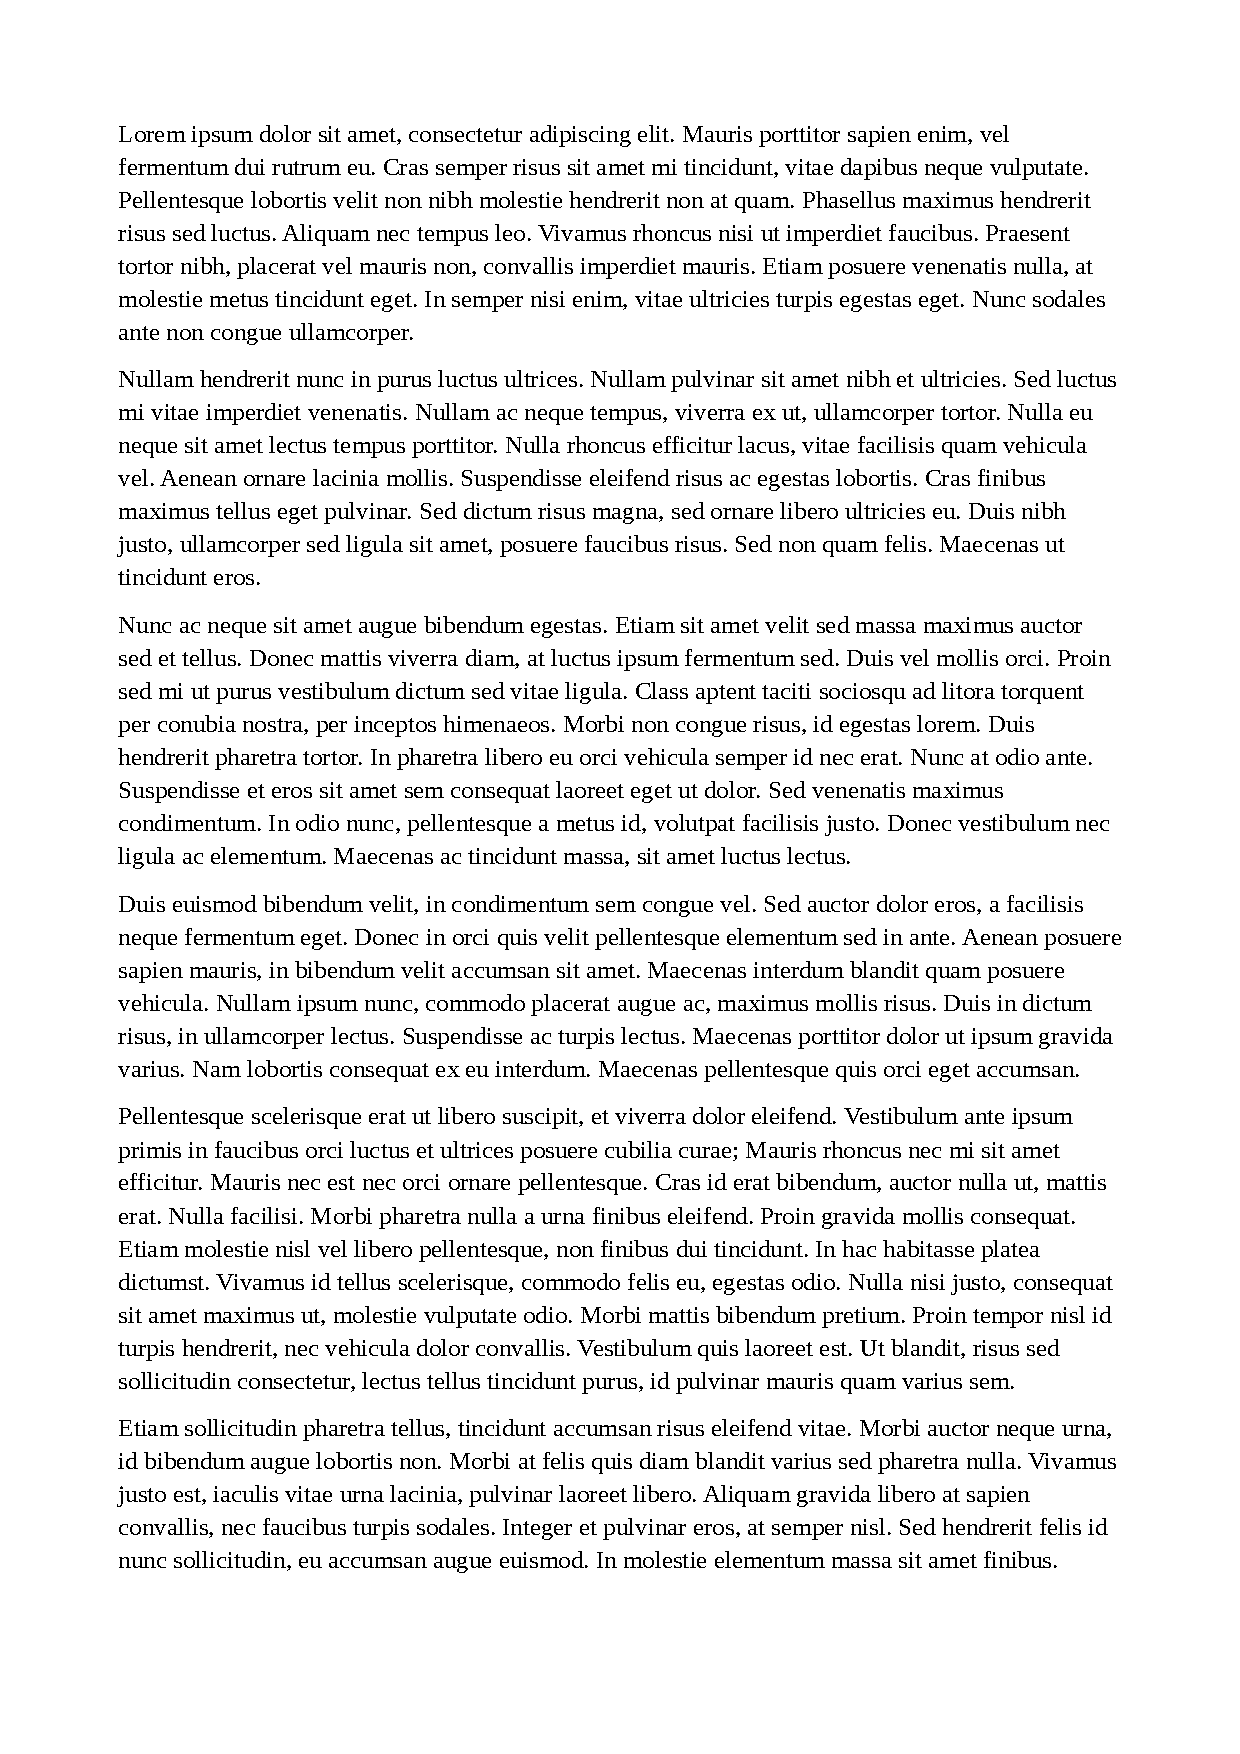
\includepdf[pages={1},scale=0.8,pagecommand=\chapter{Texto Texto Texto Texto}\label{apen:apendiceA}]{appendix/apendiceA}
\includepdf[pages={2-},scale=0.80,pagecommand={}]{appendix/apendiceA}

%coloca o identificador do anexo/apendice somente na primeira página

\includepdf[pages={1},scale=0.80,pagecommand=\chapter{Texto Texto Texto}\label{apen:apendiceB}]{appendix/apendiceB}


%coloca o identificador do anexo/apendice somente na primeira página
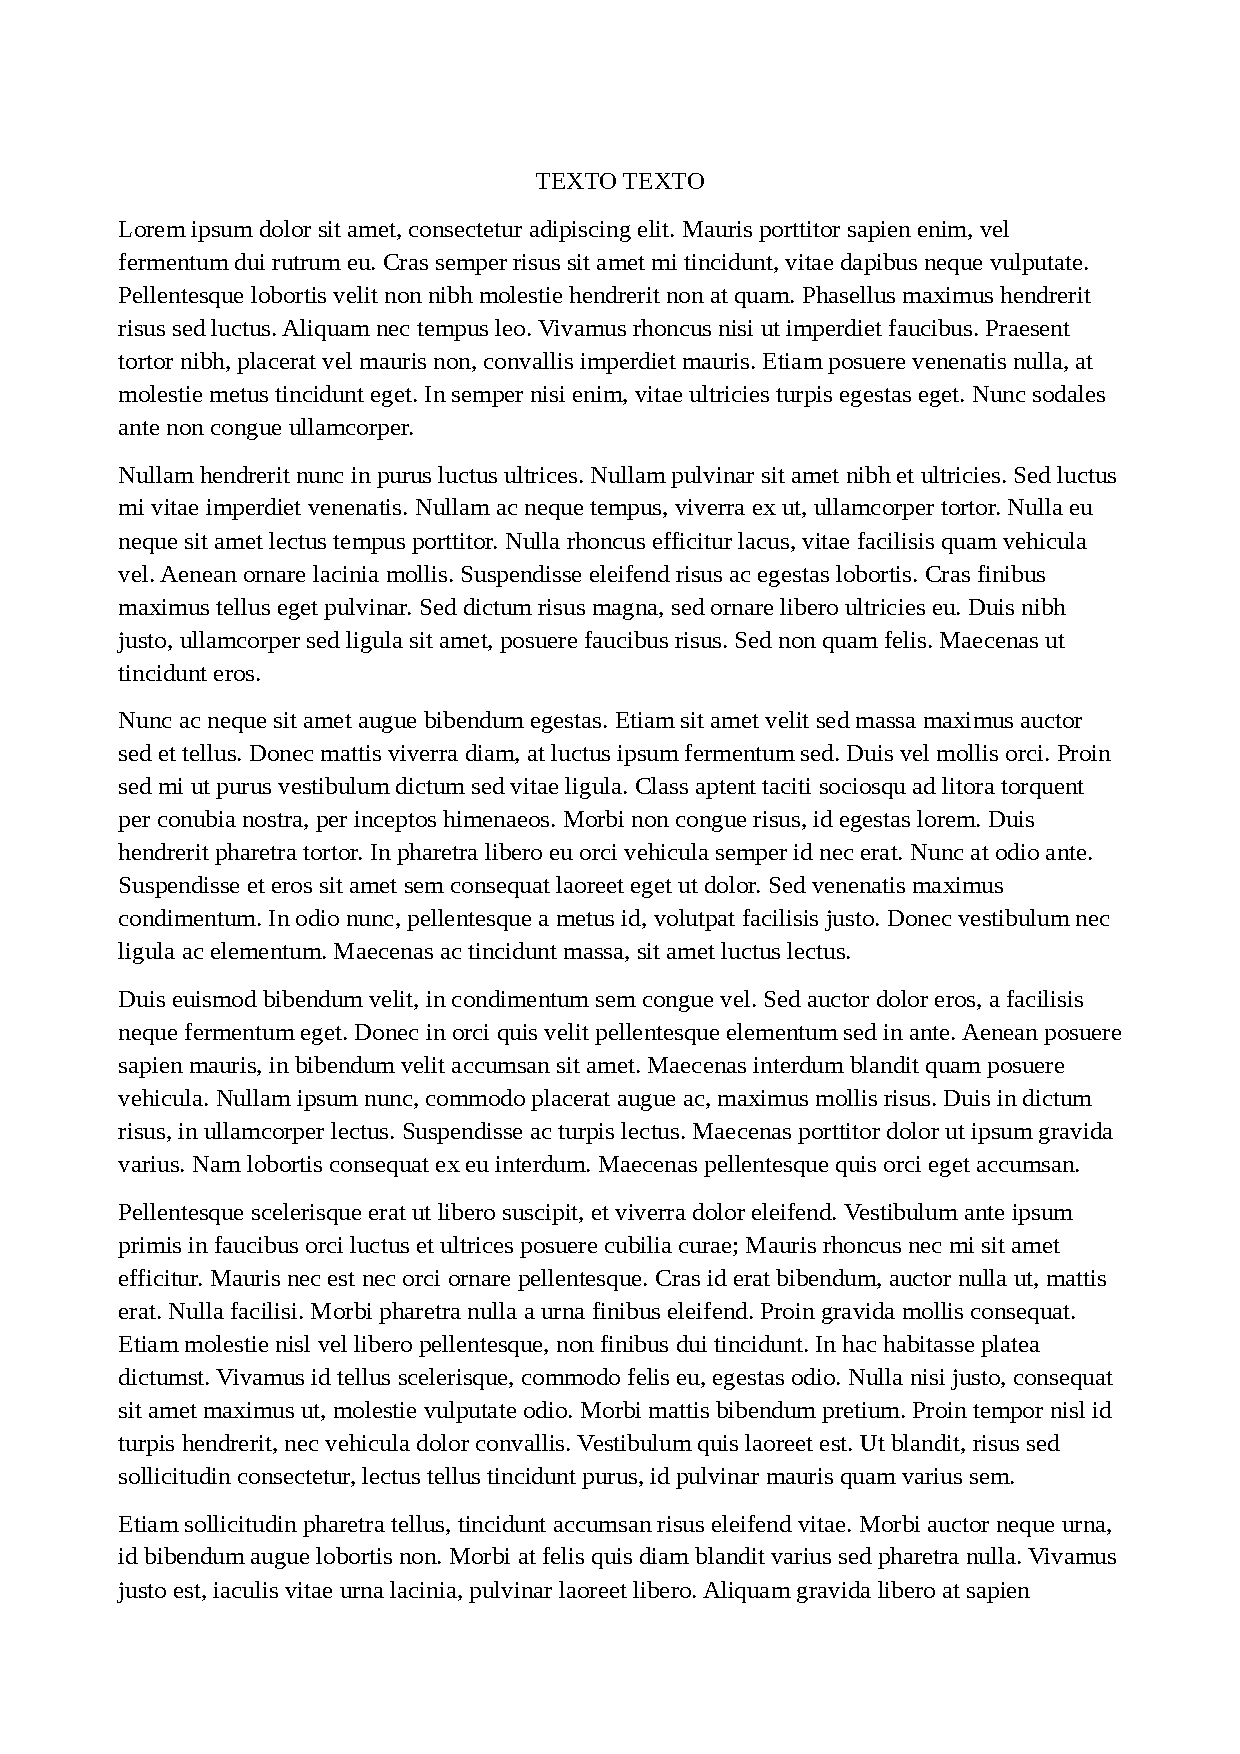
\includepdf[pages={1},scale=0.80,pagecommand=\chapter{Texto Texto}\label{apen:apendiceC}]{appendix/apendiceC}
\includepdf[pages={2},scale=0.80,pagecommand={}]{appendix/apendiceC}


\addtocontents{toc}{\endgroup}
\end{apendicesenv}




% ----------------------------------------------------------
% Anexos
% ----------------------------------------------------------
%
% ----------------------
% força para que não exiba subtítulos em apêndices no sumário
% -----------------------

\begin{anexosenv}
\addtocontents{toc}{\protect\setcounter{tocdepth}{1}}
\makeatletter
\addtocontents{toc}{%
  \begingroup
  \let\protect\l@chapter\protect\l@section
  \let\protect\l@section\protect\l@subsection
}
\makeatother
% Imprime uma página indicando o início dos apêndices
% \partapendices

%coloca o identificador do anexo/apendice somente na primeira página
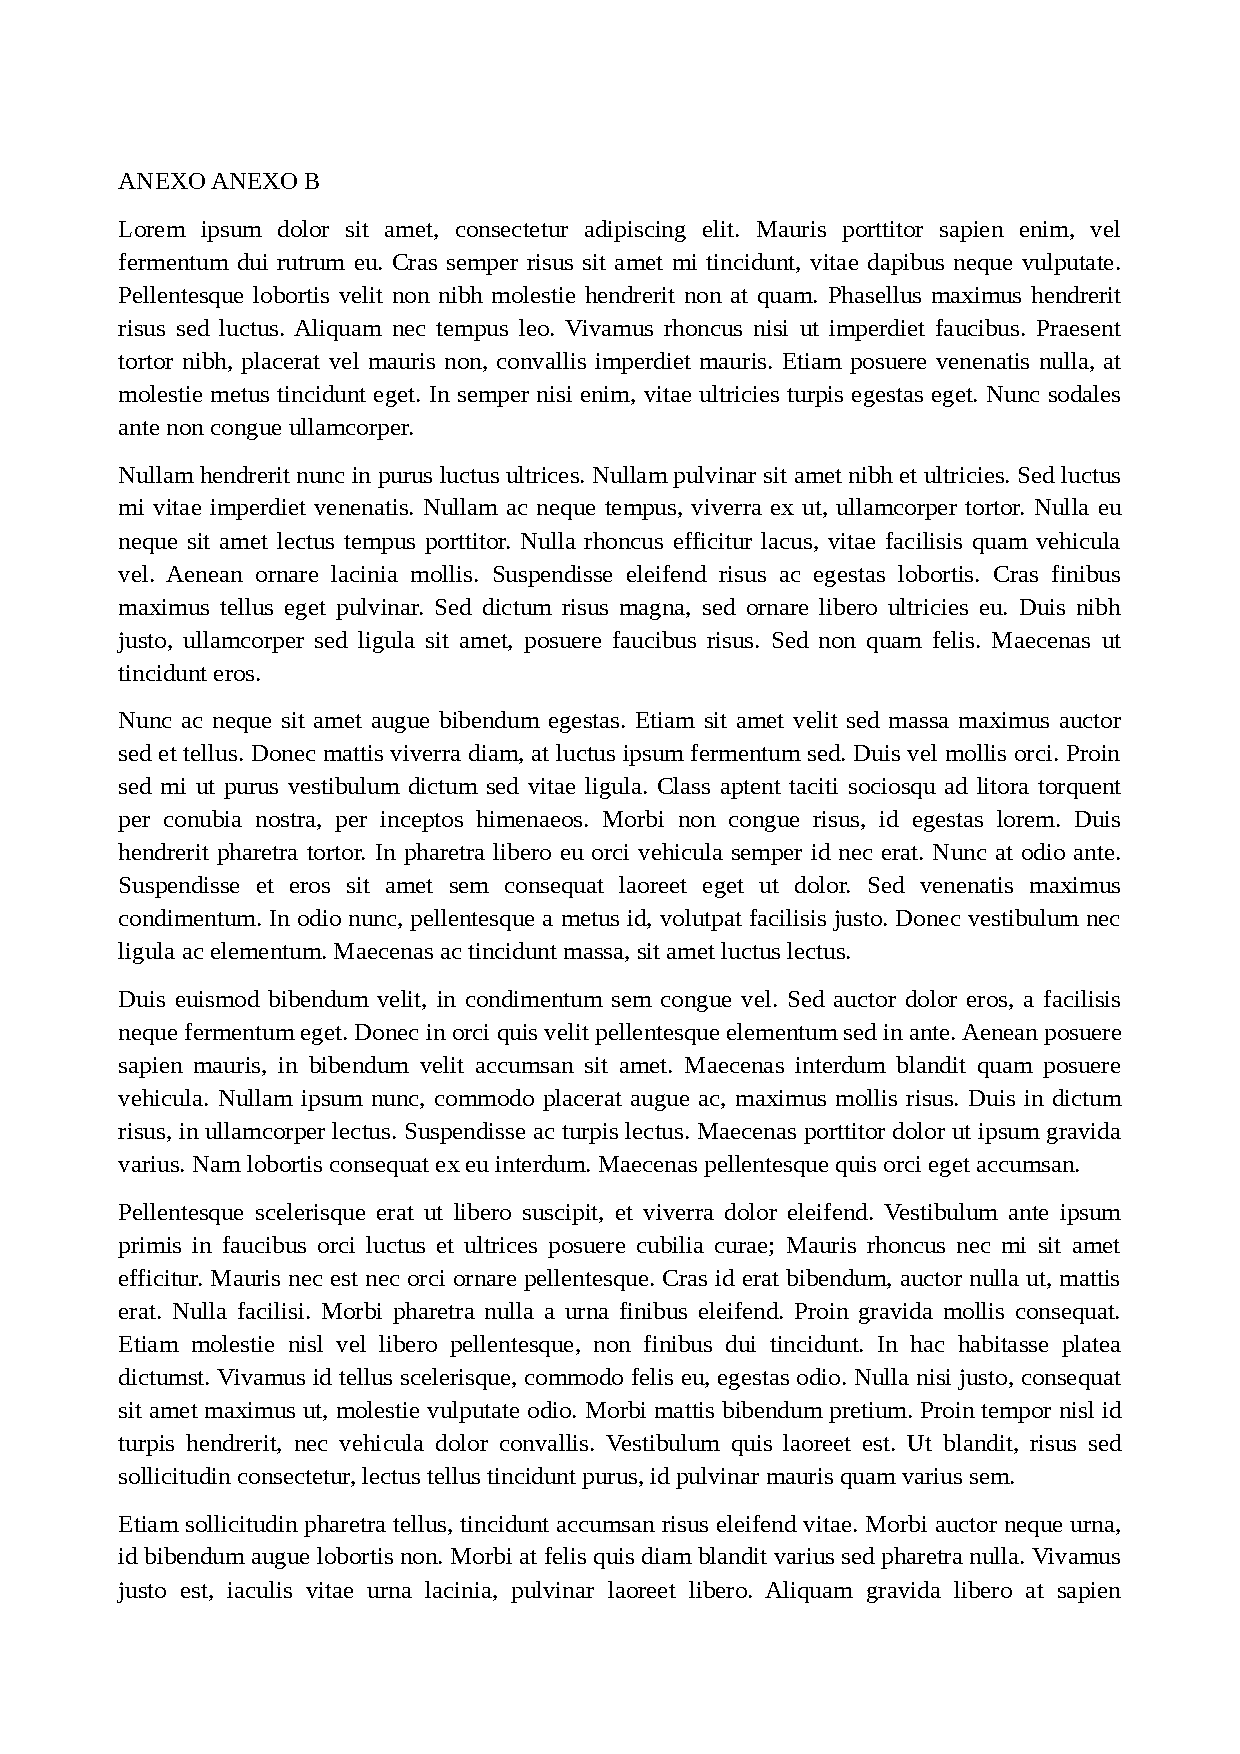
\includepdf[pages={1},scale=0.8,pagecommand=\chapter{Texto Texto Texto Texto}\label{anex:anexob}]{anexos/anexoB}
\includepdf[pages={2-},scale=0.80,pagecommand={}]{anexos/anexoB}

%coloca o identificador do anexo/apendice somente na primeira página
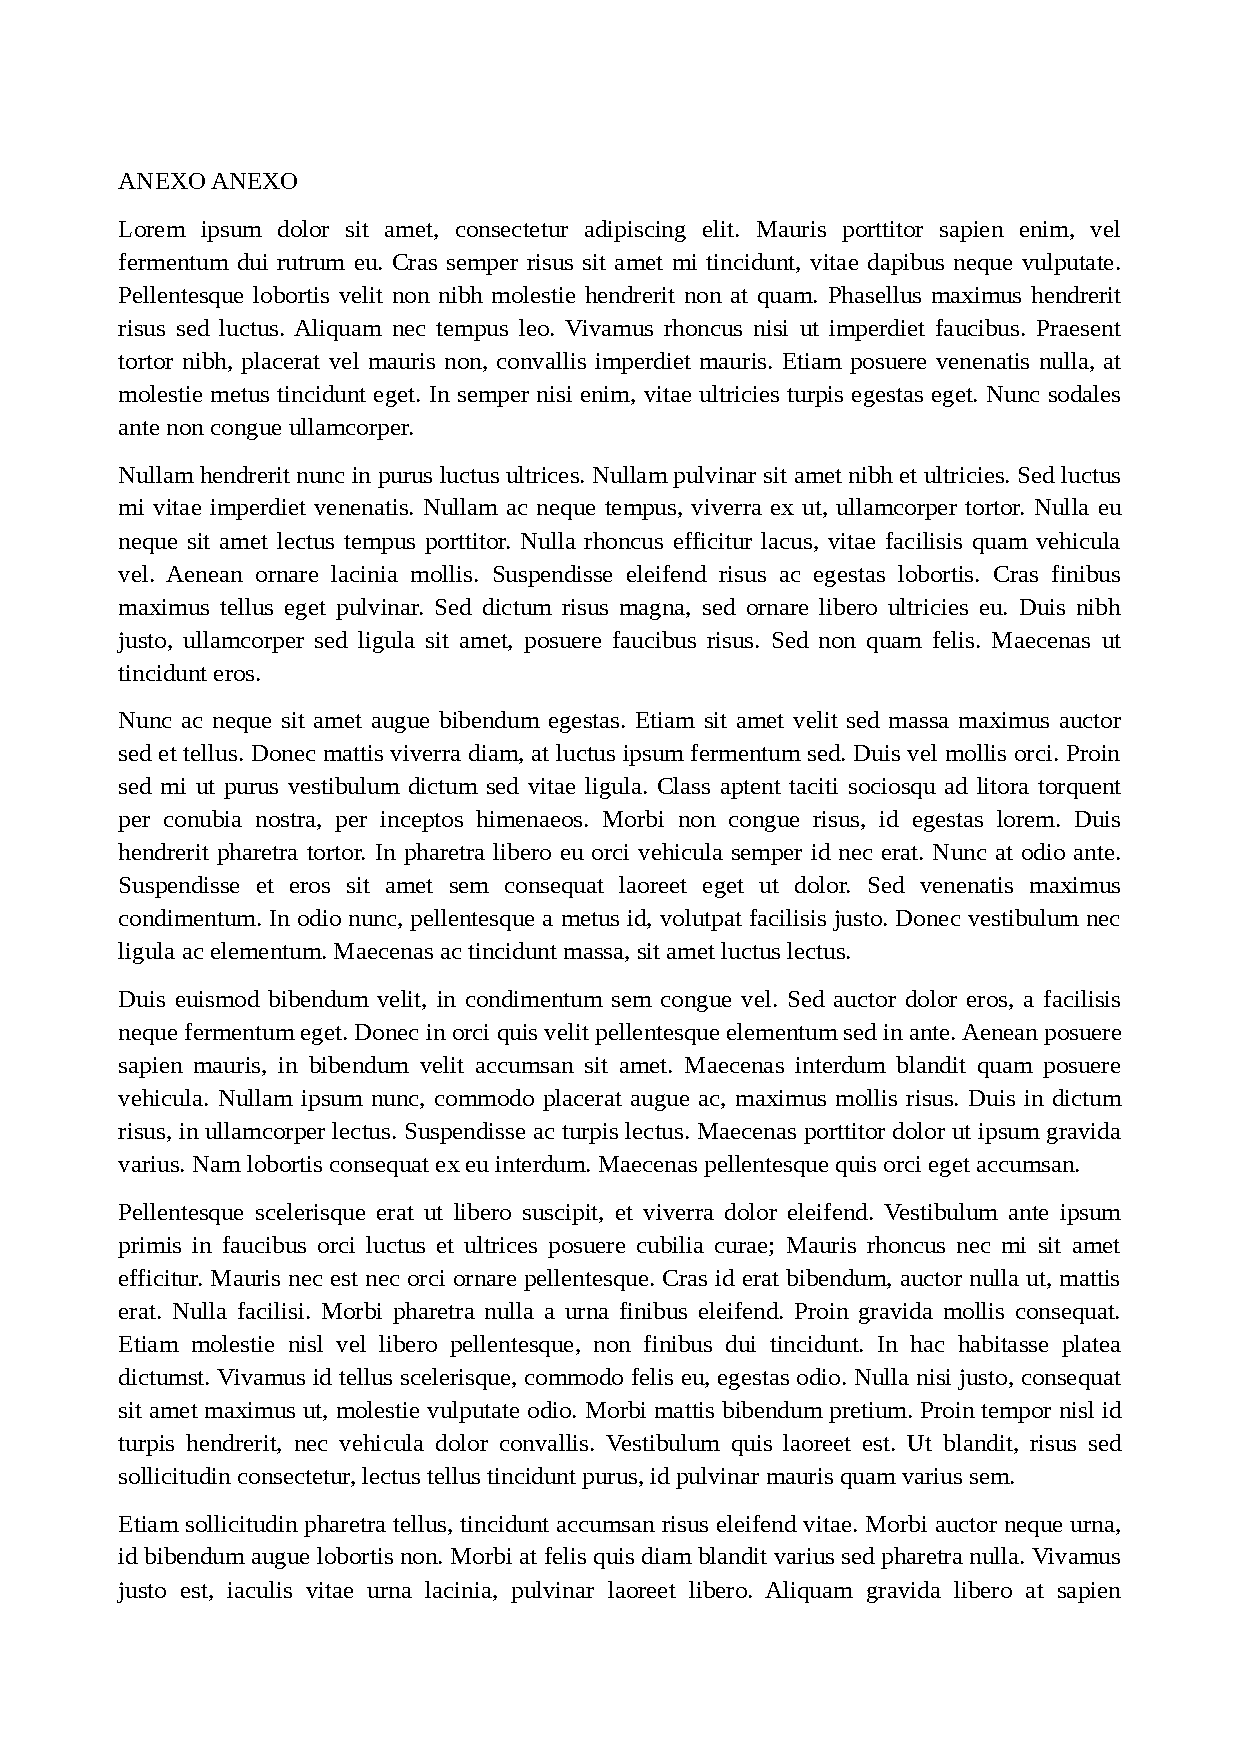
\includepdf[pages={1},scale=0.8,pagecommand=\chapter{Texto Texto Texto Texto}\label{anex:anexoa}]{anexos/anexoA}
\includepdf[pages={2-},scale=0.80,pagecommand={}]{anexos/anexoA}

\addtocontents{toc}{\endgroup}
\end{anexosenv}





\printindex


\end{document}
